%!TEX root = modelguide.tex

% Scale latexml image sizes 2x
\newlength{\imglength}
\newcommand{\setlengthLaTeXML}[3]{ %
	\iflatexml %
	\setlength{#1}{#2} %
	\else %
	\setlength{#1}{#3} %
	\fi %
}

\chapter{Finite Element Models}
\label{FEMModels:sec}

This section details how to construct three-dimensional finite element models,
and how to couple them with the other simulation components described in
previous sections (e.g.~particles and rigid bodies).  Finite element
\emph{muscles}, which have additional properties that allow them to contract
given activation signals, are discussed in Section \ref{sec:fem:muscle}.  An 
example FEM model of the masseter, coupled to a rigid jaw and maxilla, is shown 
in Figure \ref{fig:fem:masseter}.

\begin{figure}[ht]
	\centering
	\setlengthLaTeXML{\imglength}{0.8\textwidth}{0.6\textwidth}
	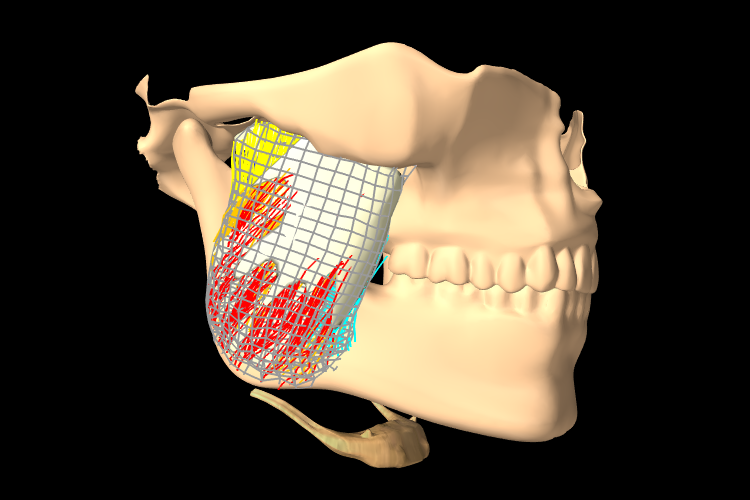
\includegraphics[width=\imglength]{images/fem_masseter}
	\caption{Finite element model of the masseter, coupled to the jaw and 
	         maxilla. \label{fig:fem:masseter}} 
\end{figure}

\section{Overview}
\label{sec:fem:overview}

The finite element method (FEM) is a numerical technique used for solving a 
system of partial differential equations (PDEs) over some domain.  The general
approach is to divide the domain into a set of building blocks, referred to
as \emph{elements}.  These partition the space, and form local domains over
which the system of equations can be locally approximated. The corners of these
elements, the \emph{nodes}, become control points in a discretized system.  
The solution is then assumed to be
smoothly interpolated across the elements based on values determined at the
nodes.  Using this discretization, the differential system is converted into 
an algebraic one, which is often linearized and solved iteratively.

In ArtiSynth, the PDEs considered are the governing equations of
continuum mechanics: the conservation of mass, momentum, and energy.  To 
complete the system, a \emph{constitutive equation} is required that describes
the stress-strain response of the material.  This constitutive equation is what
distinguishes between material types.  The domain is the three-dimensional space
that the model occupies. This must be divided into small elements which 
accurately represent the geometry. Within each element, the PDEs are
sampled at a set of points, referred to as \emph{integration points}, and 
terms are numerically integrated to form an algebraic system to solve.

The purpose of the rest of this section is to describe the construction and
use of finite elements models within ArtiSynth.  It does not further discuss 
the mathematical framework or theory.
For an in-depth coverage of the nonlinear finite element method, as applied
to continuum mechanics, the reader is referred to the textbook by Bonet and 
Wood \cite{bonet:fem:2000}.

\subsection{FemModel3d}
\label{sec:fem:structure}

The basic type of finite element model is implemented in the class 
\javaclass[artisynth.core.femmodels]{FemModel3d}.  This class controls some
properties that are used by the model as a whole.  The key ones that affect
simulation dynamics are:
\begin{center}
	\begin{tabular}{|ll|}
		\hline
		Property & Description\\
		\hline
		{\tt density} & The density of the model\\
		{\tt material} & An object that describes the material's 
		    \emph{constitutive law} (i.e.~its stress-strain relationship).\\
		{\tt particleDamping} & Proportional damping associated with the 
		    particle-like motion of the FEM nodes.\\
		{\tt stiffnessDamping} & Proportional damping associated with the 
		    system's stiffness term.\\
		\hline
	\end{tabular}
\end{center}
These properties can be set and retrieved using the methods
\begin{lstlisting}[]
	setDensity ( double density );    // sets the density
	double getDensity ();             // gets the density

	setMaterial ( FemMaterial mat );  // sets the FEM's material
	FemMaterial getMaterial ();       // gets the FEM's material

	setParticleDamping ( double d );  // sets the particle (mass) damping coefficient
	double getParticleDamping ();     // gets the particle (mass) damping coefficient

	setStiffnessDamping ( double d ); // sets the stiffness damping coefficient
	double getStiffnessDamping ( );   // gets the stiffness damping coefficient
\end{lstlisting}
Keep in mind that ArtiSynth is essentially ``unitless'' (Section 
\ref{sec:mechii:units}), so it is the responsibility of the developer to
ensure that all properties are specified in a compatible way.  

The density of the model is used to compute the mass distribution throughout
the volume.  Note that we use a \emph{diagonally lumped mass matrix} (DLMM)
formulation, so the mass is assumed to be concentrated at the location of
the discretized FEM nodes.  To allow for a spatially-varying density,
a mass can later be specified for each node individually.

The FEM's {\tt material} is a delegate object used to compute stress and 
stiffness within individual elements.  It handles the \emph{constitutive}
component of the model.  Materials will be discussed in more detail in
Section \ref{sec:fem:materials}.

The two damping parameters are related to \emph{Rayleigh damping}, which
is used to dissipate energy within finite element models.  There are two 
proportional damping terms: one related to the system's mass, and one related 
to stiffness.  The resulting damping force applied is
\begin{align}
	\f_d & = - (d_M \M + d_K\K)\v,
\end{align}
where $d_M$ is the value of {\tt particleDamping}, $d_K$ is the value of 
{\tt stiffnessDamping}, $\M$ is the FEM model's lumped mass matrix, $\K$ is 
the FEM's stiffness matrix, and $\v$ is the concatenated vector of FEM node
velocities.  Since the lumped mass matrix is diagonal, the mass-related
component of damping can be applied separately to each FEM node.  Thus, the
mass component reduces to the same system as Equation \eqref{eqn:pointdamping},
which is why it is referred to as ``particle damping''.

\subsection{Component Structure}

Each \javaclass[artisynth.core.femmodels]{FemModel3d} contains three 
lists of sub-components:

\begin{description}
\item[{\tt nodes}]\mbox{}

The particle-like dynamic components of the model.  These lie at the corners
of the elements and carry all the mass (due to DLMM formulation).

\item[{\tt elements}]\mbox{}

The spatial building blocks of the model.  These define the sub-units over 
which the system is numerically integrated.

\item[{\tt meshes}]\mbox{}

The geometry in the model.  This includes the surface mesh, and any other
embedded geometries.
\end{description}

An example showing each of these components is shown in Figure \ref{fig:fem}.

\begin{figure}[ht]
	\centering
	%\subfigure[][FEM model \label{fig:fem:model}] {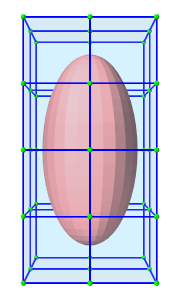
\includegraphics[width=0.2\textwidth]{images/fem_embedded.png}}
	%\subfigure[][Nodes \label{fig:fem:nodes}] {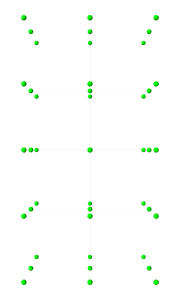
\includegraphics[width=0.2\textwidth]{images/fem_embedded_nodes.png}}
	%\subfigure[][Elements \label{fig:fem:elements}] {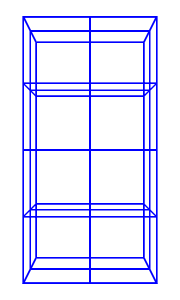
\includegraphics[width=0.2\textwidth]{images/fem_embedded_elements.png}}
	%\subfigure[][Geometry \label{fig:fem:geometry}] {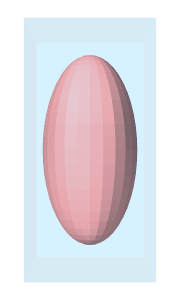
\includegraphics[width=0.2\textwidth]{images/fem_embedded_geometry.png}}
	\setlengthLaTeXML{\imglength}{1.5in}{1.2in}
	\begin{tabular}{cccc}
	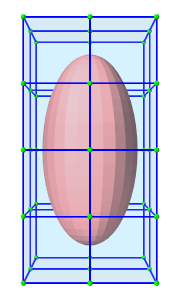
\includegraphics[width=\imglength]{images/fem_embedded.png} & 
	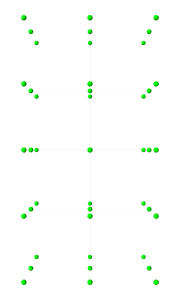
\includegraphics[width=\imglength]{images/fem_embedded_nodes.png} &
	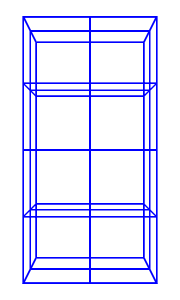
\includegraphics[width=\imglength]{images/fem_embedded_elements.png} &
	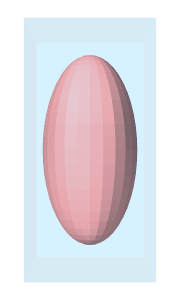
\includegraphics[width=\imglength]{images/fem_embedded_geometry.png}\\
	(a) FEM model & (b) Nodes & (c) Elements & (d) Geometry
	\end{tabular}
	\caption{Sub-components of \javaclass[artisynth.core.femmodels]{FemModel3d}. \label{fig:fem}}
\end{figure}

\paragraph{Nodes}
\ifLaTeXML{\newline}

The set of nodes belong to a finite element model can be obtained by the method
\begin{lstlisting}[]
PointList<FemNode3d> getNodes();  // returns list of FEM nodes
\end{lstlisting}
Nodes are implemented in the class 
\javaclass[artisynth.core.femmodels]{FemNode3d}, which is a subclass of 
\javaclass[artisynth.core.mechmodels]{Particle} (Section 
\ref{ParticlesAndSprings:sec}).  They are the main dynamic components of
the finite element model.  The key properties affecting simulation dynamics
are:
\begin{center}
	\begin{tabular}{|ll|}
		\hline
		Property & Description\\
		\hline
		{\tt restPosition} & The initial position of the node.\\
		{\tt position} & The current position of the node.\\
		{\tt velocity} & The current velocity of the node.\\
		{\tt mass} & The mass of the node.\\
		{\tt dynamic} & Whether the node is considered dynamic or parametric 
		                (e.g.~boundary condition).\\
		\hline
	\end{tabular}
\end{center}
Each of these properties has corresponding {\tt getXxx()} and 
{\tt setXxx(...)} functions to access and modify them.

The {\tt restPosition} property defines the node's position in the FEM model's 
``natural'' or ``undeformed'' state.  Rest positions are used to compute
an initial configuration for the model, from which strains are determined.  A
node's rest position can be updated in code using the method:
\javamethod[artisynth.core.femmodels]{FemNode3d.setRestPosition(Point3d)}.

\begin{sideblock}
If any node's rest positions are changed, the current values 
for stress and stiffness will become invalid.  They can be manually
updated using the method \javamethod[artisynth.core.femmodels] %
{FemModel3d.updateStressAndStiffness()} for the parent model. Otherwise,
stress and stiffness will be automatically updated at the beginning of the 
next time step. 
\end{sideblock}

The properties {\tt position} and {\tt velocity} give the node's current
3D state.  These are common to all point-like particles, as is the 
{\tt mass} property.  Here, however, {\tt mass} represents the lumped mass
of the immediately surrounding material.  Its value is initialized by equally
dividing mass contributions from each adjacent element, given their
densities.  For a finer control of spatially-varying density,
node masses can be set manually after FEM creation.

The FEM node's {\tt dynamic} property specifies whether or not the 
node is considered when computing the dynamics of the system.  If not,
it is treated as being parametrically controlled.  This has implications
when setting boundary conditions (Section \ref{sec:fem:boundary}).

\paragraph{Elements}
\ifLaTeXML{\newline}

Elements are the spatial building blocks of the domain.  Within each element,
the displacement (or strain) field is interpolated from displacements at nodes:
\begin{align}
	\u(\x) & = \sum_{i=1}^N \phi_i(\x)\u_i, \label{eqn:fem:interp}
\end{align}
where $\u_i$ is the displacement of the $i$th node that is adjacent to the 
element, and $\phi_i(\cdot)$ is referred to as the \emph{shape function} (or 
\emph{basis function}) associated with that node.  Elements are classified by 
their shape, number of nodes, and shape function order (Table 
\ref{tbl:fem:elements}).  ArtiSynth supports the following element types:
\begin{center}
	\setlengthLaTeXML{\imglength}{1.5in}{1in}
	\begin{tabular}{c@{\hspace{5ex}}c@{\hspace{5ex}}c@{\hspace{5ex}}c}
		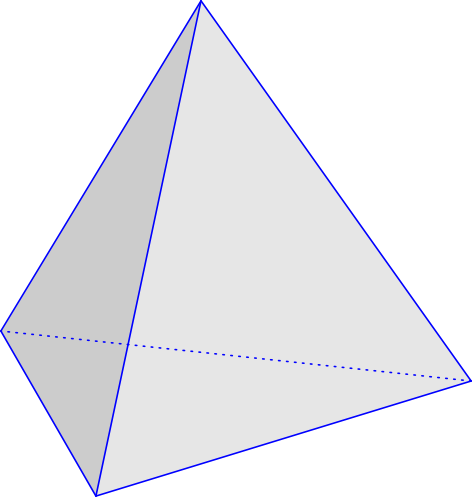
\includegraphics[height=\imglength]{images/fem_element_tet} &
		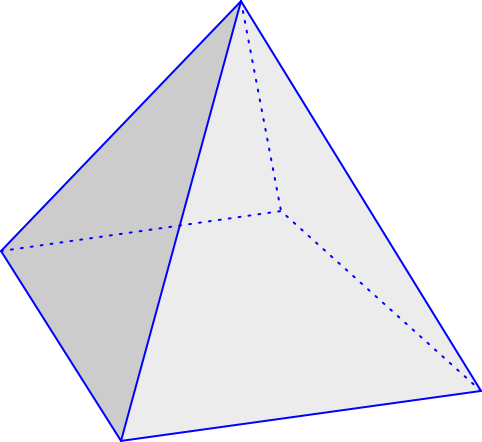
\includegraphics[height=\imglength]{images/fem_element_pyramid} &
		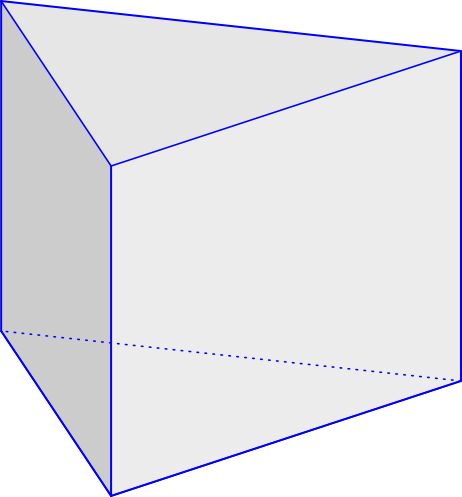
\includegraphics[height=\imglength]{images/fem_element_wedge} &
		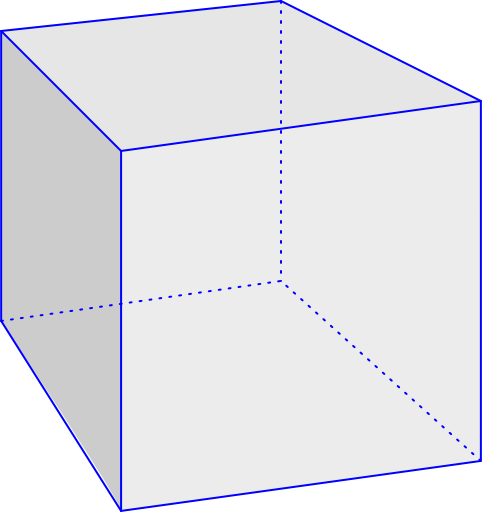
\includegraphics[height=\imglength]{images/fem_element_hex} \\
		\javaclass[artisynth.core.femmodels]{TetElement}, &
		\javaclass[artisynth.core.femmodels]{PyramidElement}, & 
		\javaclass[artisynth.core.femmodels]{WedgeElement}, &
		\javaclass[artisynth.core.femmodels]{HexElement},\\
		\javaclass[artisynth.core.femmodels]{QuadtetElement} &
		\javaclass[artisynth.core.femmodels]{QuadpyramidElement} & 
		\javaclass[artisynth.core.femmodels]{QuadwedgeElement} &
		\javaclass[artisynth.core.femmodels]{QuadhexElement}
	\end{tabular}
\end{center}
\begin{table}[ht]
\centering
\caption{Supported element types \label{tbl:fem:elements}}
\begin{tabular}{lccc}
	\hline\hline
	Element Type & \# Nodes & Order &  \# Integration Points \\
	\hline
	\javaclass[artisynth.core.femmodels]{TetElement} & 4 & linear & 1\\
	\javaclass[artisynth.core.femmodels]{PyramidElement} & 5 & linear & 5\\
	\javaclass[artisynth.core.femmodels]{WedgeElement} & 6 & linear & 6\\
	\javaclass[artisynth.core.femmodels]{HexElement} & 8 & linear & 8\\
	\javaclass[artisynth.core.femmodels]{QuadtetElement} & 10 & quadratic & 4\\
	\javaclass[artisynth.core.femmodels]{QuadpyramidElement} & 13 & quadratic & 5\\
	\javaclass[artisynth.core.femmodels]{QuadwedgeElement} & 15 & quadratic & 9\\
	\javaclass[artisynth.core.femmodels]{QuadhexElement} & 20 & quadratic & 14\\
	\hline
\end{tabular}
\end{table}
The base class for all of these is \javaclass[artisynth.core.femmodels]%
{FemElement3d}.  A numerical integration is performed within each element
to create the (tangent) stiffness matrix.  This integration is performed
by evaluating the stress and stiffness at a set of \emph{integration points}
within each element, and applying numerical quadrature.  The list of elements
in a model can be obtained with the method
\begin{lstlisting}[]
RenderableComponentList<FemElement3d> getElements();  // return the list of elements
\end{lstlisting}

All objects of type \javaclass[artisynth.core.femmodels]{FemModel3d} have the 
following properties:
\begin{center}
	\begin{tabular}{|ll|}
		\hline
		Property & Description\\
		\hline
		{\tt density} & Density of the element\\
		{\tt material} & An object that describes the \emph{constitutive law} 
		                 within the element (i.e.~its stress-strain 
		                 relationship).\\
		\hline
	\end{tabular}
\end{center}

If left unspecified, the element's {\tt density} is inherited from the 
containing {\tt FemModel3d} object.  When set, the mass of the element is
computed and divided amongst all its nodes, updating the lumped mass
matrix.

Each element's' {\tt material} property is also inherited by default from the 
containing {\tt FemModel3d}. Specifying a material here allows for spatially-%
varying material properties across the model.  Materials will be discussed
further in Section \ref{sec:fem:materials}.

\paragraph{Meshes}
\ifLaTeXML{\newline}

The geometry associated with a finite element model consists of a collection
of meshes (e.g.~\javaclass[maspack.geometry]{PolygonalMesh}, \javaclass[maspack.geometry]{PolylineMesh},
\javaclass[maspack.geometry]{PointMesh}) that move along with the
model in a way that maintains the shape function interpolation equation 
\eqref{eqn:fem:interp}
at each vertex location.  These geometries can be used for visualizations, or 
for physical interactions like collisions.  However, they have no physical 
properties themselves. FEM geometries will be discussed in more detail in 
Section \ref{sec:fem:geometry}.  The list of meshes can be obtained with the 
method
\begin{lstlisting}[]
MeshComponentList<FemMeshComp> getMeshComps();   // return the list of meshes in a FEM
\end{lstlisting}

\subsection{Materials}
\label{sec:fem:materials}

The stress-strain relationship within each element is defined by a ``material''
delegate object, implemented by a subclass of 
\javaclass[artisynth.core.materials]{FemMaterial}.  This material object is 
responsible for implementing the functions:
%
\begin{lstlisting}[]
   public void computeStress (...)  // computes the symmetric stress tensor
   public void computeTangent (...) // computes the local tangent stiffness matrix
\end{lstlisting}
%
Inputs include a deformation gradient, pressure, and a coordinate frame that
specifies potential directions of anisotropy. The default material type is 
\javaclass[artisynth.core.materials]{LinearMaterial}, where stress is related 
to strain through:
\begin{gather}
  \sigma(\x) = D\,\epsilon(\x), \label{eqn:fem:mat:linear}\\
  \text{where }\quad D = \begin{bmatrix}
	  \lambda +2\mu & \lambda & \lambda  & 0 & 0 & 0\\
	  \lambda &  \lambda +2\mu & \lambda & 0 & 0 & 0\\
	  \lambda & \lambda & \lambda +2\mu & 0 & 0 & 0\\
	  0 & 0 & 0 & \mu & 0 & 0\\
	  0 & 0 & 0 & 0 & \mu & 0\\
	  0 & 0 & 0 & 0 & 0 & \mu
        \end{bmatrix}, \quad \lambda = \dfrac{E\nu}{(1+\nu)(1-2\nu)},  \quad
      \mu = \dfrac{E}{2(1+\nu)},\notag
\end{gather}
$\sigma$ is the standard $6\times 1$ stress vector, $\epsilon$ is the 
strain vector, $E$ is the Young's Modulus, and $\nu$ is Poisson's ratio. This
linear material uses a corotational formulation, so rotations are removed
per element before computing the strain \cite{ngan:fem:2008}.  To enable or
disable this corotational formulation, use 
\javamethod[artisynth.core.materials]{LinearMaterial.setCorotated(boolean)}.

All material models, including linear and non-linear, are available in the package  
{\tt artisynth.core.materials}.  A list of common materials is provided in 
Table \ref{tbl:fem:materials}.  Those that are subclasses of 
\javaclass[artisynth.core.materials]{IncompressibleMaterial} allow for 
incompressibility.

\begin{table}[ht]
	\centering
 	\caption{Commonly used FEM materials \label{tbl:fem:materials}}
 	\begin{tabular}{|lll|}
 		\hline
 		\hline
 		Material & Parameters & \\
 		\hline
 		\javaclass[artisynth.core.materials]{LinearMaterial} & $E$ & Young's modulus \\
 		& $\nu$ & Poisson's ratio\\
 		& corotated & corotational formulation\\
 		\hline
 		\javaclass[artisynth.core.materials]{StVenantKirchoffMaterial} & $E$ & Young's modulus\\
 		& $\nu$ & Poisson's ratio\\
 		\hline
 		\javaclass[artisynth.core.materials]{NeoHookeanMaterial} & $E$ & Young's modulus\\
 		& $\nu$ & Poisson's ratio\\
 		\hline
 		\javaclass[artisynth.core.materials]{IncompNeoHookeanMaterial} & $G$ & shear modulus\\
 		& $\kappa$ & bulk modulus\\
 		\hline
 		\javaclass[artisynth.core.materials]{MooneyRivlinMaterial} & $C_{10},C_{01},C_{20},C_{02}$ & distortional parameters\\
 		& $\kappa$ & bulk modulus\\
 		\hline
 		\javaclass[artisynth.core.materials]{OgdenMaterial} & $\mu_1,\ldots,\mu_6$ & material parameters\\
 		& $\alpha_1,\ldots,\alpha_6$ &\\
 		& $\kappa$ & bulk modulus\\
		\hline
	\end{tabular}
\end{table}


\subsection{Boundary conditions}
\label{sec:fem:boundary}

Boundary conditions can be implemented in one of several ways:
\begin{enumerate}
	\item Explicitly setting FEM node positions/velocities
	\item Attaching FEM nodes to other dynamic components
	\item Enabling collisions
\end{enumerate}
To enforce an explicit (Dirichlet) boundary condition for a set of  
nodes, their {\tt dynamic} property must be set to {\tt false}.  This notifies
ArtiSynth that the state of these nodes (both position and velocity) will 
be controlled parametrically.  By disabling dynamics, a fixed 
boundary condition is applied.  For a moving boundary, positions and velocities 
of the boundary nodes must be explicitly set every timestep.  This can be 
accomplished with either a \javaclass[artisynth.core.modelbase]{Controller} 
(see Section \ref{ControllersAndMonitors:sec}) or an 
\javaclass[artisynth.core.probes]{InputProbe} (see Section \ref{Probes:sec}).
Note that both the position \emph{and} velocity of the nodes should be
explicitly set for consistency.

Another type of supported boundary condition is to attach FEM nodes to other
components, including particles, springs, rigid bodies, and locations within
other FEM elements.  Here, the node is still considered dynamic, but its
motion is coupled to that of the attached component through a constraint
mechanism. Attachments will be discussed further in Section 
\ref{sec:fem:nodeattachments}.

Finally, the boundary of a FEM can be constrained by enabling collisions
with other components.  This will be covered in Section
\ref{sec:fem:collision}.


\section{FEM model creation}

Creating a finite element model in ArtiSynth typically follows the pattern:
\begin{lstlisting}[]
   // Create and add main MechModel
   MechModel mech = new MechModel("mech");
   addModel(mech);
      
   // Create FEM
   FemModel3d fem = new FemModel3d("fem");
   
   /* ... Setup FEM structure and properties ... */
   
   // Add FEM to model
   mech.addModel(fem); 
\end{lstlisting}
The main code block for the FEM setup should do the following:
\begin{itemize}
	\setlength{\itemsep}{-0.3em}
	\item Build the node/element structure
	\item Set physical properties%
	\ifLaTeXMLelse{}{\vspace{-0.5em}}
	\begin{itemize}
		\setlength{\itemsep}{-0.3em}
		\item density
		\item damping
		\item material
	\end{itemize} 
	\item Set boundary conditions
	\item Set render properties
\end{itemize}
Building the FEM structure can be done with the use of factory
methods for simple shapes, by loading external files, or by writing code
to manually assemble the nodes and elements.

\subsection{Factory methods}

For simple shapes such as beams and ellipsoids, there are factory methods to 
automatically build the node and element structure.  These methods are found
in the \javaclass[artisynth.core.femmodels]{FemFactory} class.  Some common
methods are
\begin{lstlisting}[]
FemFactory.createGrid(...)          // basic beam
FemFactory.createCylinder(...)      // cylinder
FemFactory.createTube(...)          // hollowed cylinder
FemFactory.createEllipsoid(...)     // ellipsoid
FemFactory.createTorus(...)         // torus
\end{lstlisting}
The inputs specify the dimensions, resolution, and potentially the type
of element to use.  The following code creates a basic beam made up of
hexahedral elements:
\begin{lstlisting}[]
// Create FEM
FemModel3d beam = new FemModel3d("beam");
      
// Build FEM structure
double[] size = {1.0, 0.25, 0.25};  // widths
int[] res = {8, 2, 2};              // resolution (# elements)
      
FemFactory.createGrid(beam, FemElementType.Hex,
	size[0], size[1], size[2], 
	res[0], res[1], res[2]);

/* ... Set FEM properties ... */

// Add FEM to model
mech.addModel(beam);
\end{lstlisting}

\subsection{Loading external FEM meshes}

For more complex geometries, volumetric meshes can be loaded from external
files.  A list of supported file types is provided in Table 
\ref{tbl:fem:fileformats}. To load a geometry, an appropriate file reader
must be created.  Readers capable of reading FEM models implement the 
interface \javaclass[artisynth.core.femmodels]{FemReader}, which has the
method
\begin{lstlisting}[]
readFem( FemModel3d fem )   // populates the FEM based on file contents
\end{lstlisting}
Additionally, many {\tt FemReader} classes have static methods to handle
the loading of files for convenience.

\begin{table}[ht]
	\centering
	\caption{Supported FEM geometry files \label{tbl:fem:fileformats}}
	\begin{tabular}{llll}
		\hline\hline
		Format & File extensions & Reader & Writer\\
		\hline
		ANSYS & .node, .elem & \javaclass[artisynth.core.femmodels]{AnsysReader} & \javaclass[artisynth.core.femmodels]{AnsysWriter}\\
		TetGen & .node, .ele & \javaclass[artisynth.core.femmodels]{TetGenReader} & \javaclass[artisynth.core.femmodels]{TetGenWriter}\\
		Abaqus & .inp & \javaclass[artisynth.core.femmodels]{AbaqusReader} & \javaclass[artisynth.core.femmodels]{AbaqusWriter}\\
		VTK (ASCII) & .vtk & \javaclass[artisynth.core.femmodels]{VtkAsciiReader} & \multicolumn{1}{c}{--}\\
		\hline
	\end{tabular}
\end{table}

The following code snippet demonstrates how to load a model using the
\javaclass[artisynth.core.femmodels]{AnsysReader}.
\begin{lstlisting}[]
// Create FEM
FemModel3d tongue = new FemModel3d("tongue");
      
// Read FEM from file
try {
   // Get files relative to THIS class
   String nodeFileName = ArtisynthPath.getSrcRelativePath(this, 
                            "data/tongue.node");
   String elemFileName = ArtisynthPath.getSrcRelativePath(this, 
                            "data/tongue.elem");

   AnsysReader.read(tongue, nodeFileName, elemFileName);

} catch (IOException ioe) {         
   // Wrap error, fail to create model
   throw new RuntimeException("Failed to read model", ioe);
}
      
// Add to model
mech.addModel(tongue);
\end{lstlisting}
The method \javamethod[artisynth.core.util]{ArtisynthPath.getSrcRelativePath()}
is used to find a path within the ArtiSynth source tree that is relative to the
current model's source file.  Note the try-catch block.  Most of these readers 
throw an {\tt IOException} if the read fails.

\subsection{Generating from surfaces}

There are two ways a FEM model can be generated from a surface: by using a
FEM mesh generator, and by extruding a surface along its normal direction.

ArtiSynth has the ability to interface directly with the TetGen library 
(\href{http://tetgen.org}{http://tetgen.org}) to create a tetrahedral 
volumetric mesh given a closed and manifold surface.  The main Java class for
calling TetGen directly is \javaclass[maspack.geometry]{TetgenTessellator}.
The tessellator has several advanced options, allowing for the computation of 
convex hulls, and for adding points to a volumetric mesh.  For simply creating
a FEM from a surface, there is a convenience routine within 
\javaclass[artisynth.core.femmodels]{FemFactory} that handles both mesh 
generation and constructing a {\tt FemModel3d}:
\begin{lstlisting}[]
// Create a FEM from a manifold mesh with a given quality
FemFactory.createFromMesh( PolygonalMesh mesh, double quality );
\end{lstlisting}
If {\tt quality} $>0$, then points will be added in an attempt to bound the
maximum radius-edge ratio (see the {\tt-q} switch for TetGen).  According
to the TetGen documentation, the algorithm \emph{usually} succeeds for a 
quality ratio of 1.2.

It's also possible to create thin layer of elements by extruding a surface
along its normal direction. 
\begin{lstlisting}[]
// Create a FEM by extruding a surface
FemFactory.createExtrusion(
      FemModel3d model, int nLayers, double layerThickness, double zOffset, 
      PolygonalMesh surface);
\end{lstlisting}
For example, to create a two-layer slice of elements centered about a 
surface of a tendon mesh, one might use
\begin{lstlisting}[]
// Load the tendon surface mesh
PolygonalMesh tendonSurface = new PolygonalMesh("tendon.obj");

// Create the tendon
FemModel3d tendon = new FemModel3d("tendon");
int layers = 2;             // 2 layers
double thickness = 0.0005;  // 0.5 mm layer thickness
double offset = thickness;  // center the layers about the surface

// Create the extrusion
FemFactory.createExtrusion( tendon, layers, thickness, offset, tendonSurface );
\end{lstlisting} 
For this type of extrusion, triangular faces become wedge elements, and 
quadrilateral faces become hexahedral elements.  

\begin{sideblock}
Note: for extrusions, no care is taken to ensure element quality; if the 
surface has a high curvature relative to the total extrusion thickness, 
then some elements will be inverted.
\end{sideblock}

\subsection{Building elements in code}

A finite element model's structure can also be manually constructed in code.  
\javaclass[artisynth.core.femmodels]{FemModel3d} has the methods:
\begin{lstlisting}[]
addNode ( FemNode3d );       // add a node to the model
addElement ( FemElement3d )  // add an element to the model
\end{lstlisting}
For an element to successfully be added, all its nodes must already have
been added to the model.  Nodes can be constructed from a 3D location, and
elements from an array of nodes.  A convenience routine is available in
\javaclass[artisynth.core.femmodels]{FemElement3d} that automatically creates
the appropriate element type given the number of nodes (Table 
\ref{tbl:fem:elements}):
\begin{lstlisting}[]
// Creates an element using the supplied nodes
FemElement3d FemElement3d.createElement( FemNode3d[] nodes );
\end{lstlisting}
Be aware of node orderings when supplying nodes.  For linear elements, 
ArtiSynth uses a clockwise convention with respect to the outward
normal for the first face, followed by the opposite node(s).  To determine the
correct ordering for a particular element, check the coordinates returned by 
the function 
\javamethod*[artisynth.core.femmodels]{FemElement3d.getNodeCoords()}.
This returns the concatenated coordinate list for an ``ideal'' element of
the given type.

\subsection{Example: a simple beam model}
\label{sec:fem:example:fembeam}

\begin{figure}[ht]
	\centering
	\setlengthLaTeXML{\imglength}{0.8\textwidth}{0.6\textwidth}
	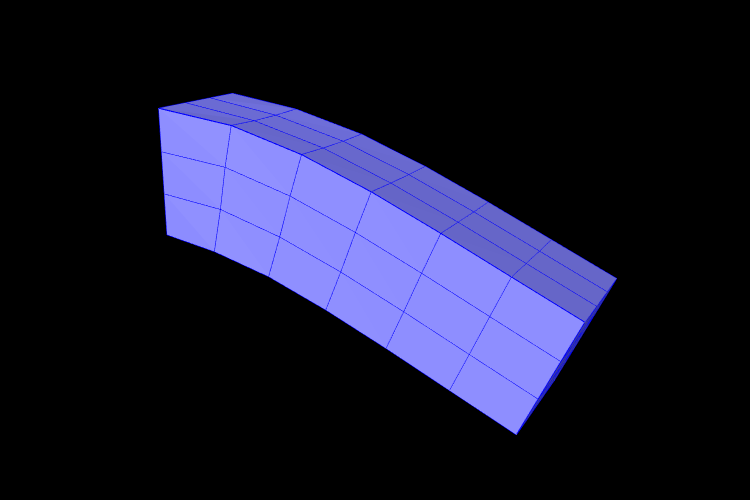
\includegraphics[width=\imglength]{images/FemBeam}
	\caption{FemBeam model loaded into ArtiSynth.}
	\label{fig:fem:beam}
\end{figure}

A complete application model that implements a simple FEM beam is given below.
\lstset{numbers=left}
\lstinputlisting{../../src/artisynth/demos/tutorial/FemBeam.java}
\lstset{numbers=none}
This example can be found in {\tt artisynth.demos.tutorial.FemBeam}.  The 
{\tt build()} method first creates a {\tt MechModel} and {\tt FemModel3d}.
A FEM beam is created using a factory method on line 36.  This beam is
centered at the origin, so its length extends from {\tt-length/2} to 
{\tt length/2}.  The density, damping and material properties are then 
assigned.  

On lines 45--49, a fixed boundary condition is set to the left-hand side 
of the beam by setting the corresponding nodes to be non-dynamic.  Due to 
numerical precision, a small {\tt EPSILON} buffer is required to ensure 
all left-hand boundary nodes are identified (line 46).

Rendering properties are then assigned to the FEM model on line 52.  These 
will be discussed further in Section \ref{sec:fem:rendering}.

\section{FEM Geometry}
\label{sec:fem:geometry}

Associated with each FEM model is a list of geometry with the heading 
{\tt meshes}.  This geometry can be used for either display purposes, 
or for interactions such as collisions.  A geometry itself has no 
physical properties; its motion is entirely governed by the FEM model 
that contains it.  

All FEM geometries are of type \javaclass[artisynth.core.femmodels]{FemMeshComp}, 
which stores a reference to a mesh object (Section \ref{Meshes:sec}), as well
as attachment information that links vertices of the mesh to points within
the FEM.  The attachments enforce the shape function interpolation in Equation
\eqref{eqn:fem:interp} to hold at each mesh vertex, with constant shape function
coefficients.

\subsection{Surface meshes}

By default, every {\tt FemModel3d} has an auto-generated geometry representing
the ``surface mesh''.  The surface mesh consists of all un-shared element faces
(i.e.~the faces of individual elements that are exposed to the world), and its
vertices correspond to the nodes that make up those faces.  As the FEM nodes
move, so do the mesh vertices due to the attachment framework.

The surface mesh can be obtained using one of the following functions in 
{\tt FemModel3d}:
\begin{lstlisting}[]
FemMeshComp getSurfaceMeshComp ();     // returns the FemMeshComp surface component
PolygonalMesh getSurfaceMesh ();  // returns the underlying polygonal surface mesh
\end{lstlisting}
The first returns the surface complete with attachment information.  The latter 
method directly returns the {\tt PolygonalMesh} that is controlled by the FEM.  

It is possible to manually set the surface mesh:
\begin{lstlisting}[]
setSurfaceMesh ( PolygonalMesh surface );  // manually set surface mesh
\end{lstlisting}
However, doing so is normally not necessary.  It is always possible to add
additional mesh geometries to a finite element model, and the visibility
settings can be changed so that the default surface mesh is not rendered.  

\subsection{Embedding geometry within an FEM}

Any geometry of type \javaclass[maspack.geometry]{MeshBase} can be added to
a {\tt FemModel3d}.  To do so, first position the mesh so that its vertices 
are in the desired locations inside the FEM, then call one of the 
{\tt FemModel3d} methods:
\begin{lstlisting}[]
FemMeshComp addMesh ( MeshBase mesh );                // creates and returns FemMeshComp
FemMeshComp addMesh ( String name, MeshBase mesh );
\end{lstlisting}
The latter is a convenience routine that also gives the newly embedded
{\tt FemMeshComp} a name.

\subsection{Example: a beam with an embedded sphere}

\begin{figure}[ht]
	\centering
	\setlengthLaTeXML{\imglength}{0.8\textwidth}{0.6\textwidth}
	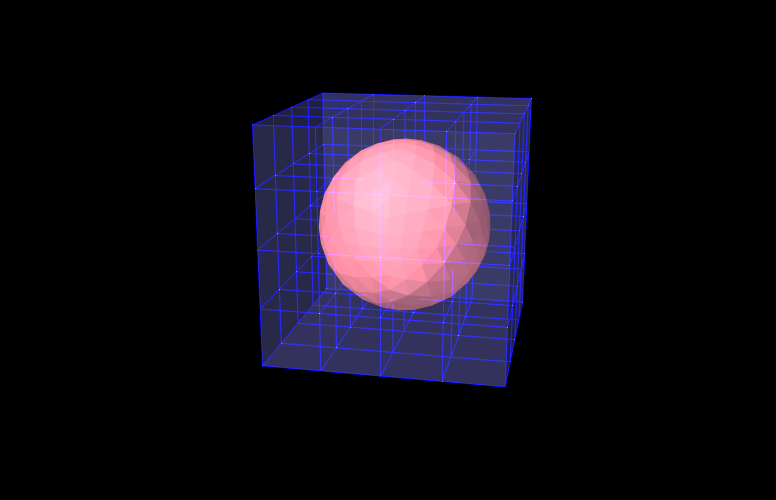
\includegraphics[width=\imglength]{images/FemEmbeddedSphere}
	\caption{FemEmbeddedSphere model loaded into ArtiSynth.}
	\label{fig:fem:embedded}
\end{figure}

A complete model demonstrating embedding a mesh is given below.
\lstset{numbers=left}
\lstinputlisting{../../src/artisynth/demos/tutorial/FemEmbeddedSphere.java}
\lstset{numbers=none}
This example can be found in {\tt artisynth.demos.tutorial.FemEmbeddedSphere}.
The model is very similar to {\tt FemBeam}.  A {\tt MechModel} and 
{\tt FemModel3d} are created and added.  At line 41, a {\tt PolygonalMesh}
of a sphere is created using a factory method.  The sphere is already
centered inside the beam, so it does not need to be repositioned.  At Line
42, the sphere is embedded inside model {\tt fem}, creating a {\tt FemMeshComp}
with the name ``sphere''.  The full model is shown in Figure 
\ref{fig:fem:embedded}.

\section{Node attachments}
\label{sec:fem:nodeattachments}

To couple FEM models to other dynamic components, the ``attachment''
mechanism described in Section \ref{PhysicsSimulation:sec} is used.
This involves creating and adding to the model attachment components,
which are instances of \javaclass[artisynth.core.mechmodels]{DynamicAttachment},
as described in Section \ref{Attachments:sec}.  
Common point-based
attachment classes are listed in Table \ref{tbl:fem:pointattachments}.

\begin{table}[ht]
	\centering
	\caption{Point-based attachments \label{tbl:fem:pointattachments}}

	\begin{tabular}{ll}
		\hline
		\hline
		Attachment & Description \\
		\hline
		\javaclass[artisynth.core.mechmodels]{PointParticleAttachment} & Attaches one ``point'' to one ``particle''\\
		\javaclass[artisynth.core.mechmodels]{PointFrameAttachment} & Attaches one ``point'' to one ``frame''\\
		\javaclass[artisynth.core.femmodels]{PointFem3dAttachment} &  Attaches one ``point'' to a linear combination of FEM nodes\\
		\hline
	\end{tabular}
\end{table}

FEM models are connected to other model components by attaching their
nodes to various components. This can be done by creating
an attachment object of the appropriate type, and then 
adding it to the {\tt MechModel} using
\begin{lstlisting}[]
  addAttachment (DynamicAttachment attach); // adds an attachment constraint
\end{lstlisting}
There are also convenience routines inside {\tt MechModel} that will create
the appropriate attachments automatically (see Section 
\ref{sec:mech:pointattachments}).

\subsection{Connecting nodes to rigid bodies or particles}

Since
\javaclass[artisynth.core.femmodels]{FemNode3d} is a subclass of
\javaclass[artisynth.core.mechmodels]{Particle}, the same methods
described in Section \ref{sec:mech:pointattachments} for attaching 
particles to other particles and frames are available. For example, 
we can attach an FEM node to a rigid body using a
either a statement of the form
%
\begin{lstlisting}[]
   mech.addAttachment (new PointFrameAttachment(body, node));
\end{lstlisting}
%
or the following equivalent statement which does the same thing:
%
\begin{lstlisting}[]
   mech.attachPoint (node, body);
\end{lstlisting}
%
Both of these create a {\tt PointFrameAttachment} between a rigid body (called
{\tt body}) and an FEM node (called {\tt node}) and then adds it to
the {\tt MechModel} {\tt mech}.

One can also attach the nodes of one FEM model to the nodes of another
using statements like
%
\begin{lstlisting}[]
   mech.addAttachment (new PointParticle (node1, node2));
\end{lstlisting}
%
or
%
\begin{lstlisting}[]
   mech.attachPoint (node2, node1);
\end{lstlisting}
%
which attaches {\tt node2} to {\tt node1}.

\subsection{Example: connecting a beam to a block}

\begin{figure}[ht]
	\centering
	\setlengthLaTeXML{\imglength}{0.8\textwidth}{0.6\textwidth}
	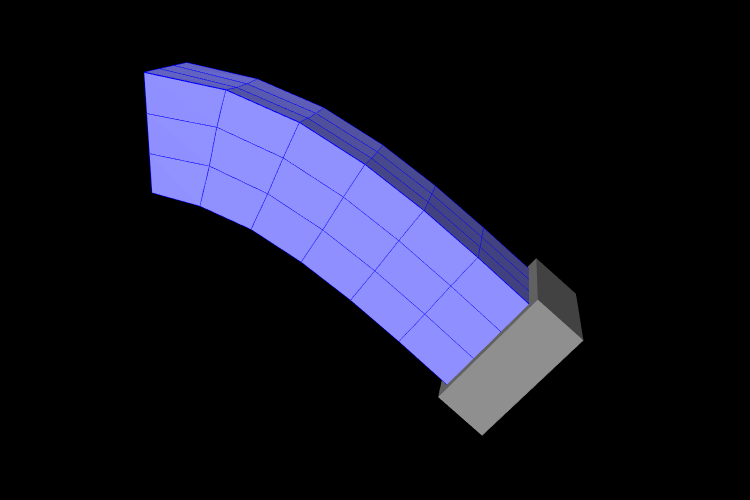
\includegraphics[width=\imglength]{images/FemBeamWithBlock}
	\caption{FemBeamWithBlock model loaded into artisynth.}
	\label{fig:fem:beamwithblock}
\end{figure}

The following model demonstrates attaching a FEM beam to a rigid block.
\lstset{numbers=left}
\lstinputlisting{../../src/artisynth/demos/tutorial/FemBeamWithBlock.java}
\lstset{numbers=none}
This model extends the {\tt FemBeam} example of Section 
\ref{sec:fem:example:fembeam}.  The {\tt build()} method then creates 
and adds a {\tt RigidBody} block (lines 18--20).  On line 21, the block
is repositioned to the side of the beam to prepare for the attachment.
On lines 24--28, all right-most nodes of the beam are then set to be attached
to the block using a {\tt PointFrameAttachment}.  In this case, the 
attachments are explicitly created.  They could also have been attached using
\begin{lstlisting}[]
   mech.attachPoint (node, block);  // attach node to rigid block
\end{lstlisting}

\subsection{Connecting nodes directly to elements}

Typically, nodes do not align in a way that makes it
possible to connect them to other FEM models and/or points based on
simple point-to-node attachments.  Instead, we use a different
mechanism that allows us to attach a point to an arbitrary location
within a FEM model. This is done using an attachment component of
type
\javaclass[artisynth.core.femmodels]{PointFem3dAttachment}, which
implements an attachment where the position $\p$ and velocity $\u$ of the
attached point is determined by a weighted sum of the positions $\p_k$ 
and velocities $\u_k$ of selected fem nodes:
%
\begin{equation}
\p = \sum w_k \p_k
\label{pointFemAttachment:eqn}
\end{equation}
%
Any force $\f$ acting on the attached point is then propagated back
to the nodes, according to the relation
%
\begin{equation}
\f_k = w_k \f
\label{pointFemForces:eqn}
\end{equation}
%
where $\f_k$ is the force acting on node $k$ due to $\f$.  This
relation can be derived based on the conservation of energy.
If $\p$ is embedded within a single element, then the $\p_k$ are
simply the element nodes and the $w_i$ are corresponding shape
function values; this is known as an {\it element-based} attachment.
On the other hand, as desribed below, it is sometimes desirable to
form an attachment using a more general set of nodes that extends
beyond a single element; this is known as a {\it nodal-based}
attachment (Section \ref{sec:fem:nodalAttachments}).

An element-based attachment can be created using a code fragment
of the form
%
\begin{lstlisting}[]
   PointFem3dAttachment ax = new PointFem3dAttachment(pnt);
   ax.setFromElement (pnt.getPosition(), elem);
   mech.addAttachment (ax);
\end{lstlisting}
%
First, a {\tt PointFem3dAttachment} is created for the point {\tt
pnt}. Next, {\tt setFromElement()} is used to determine the nodal
weights within the element {\tt elem} for the specified position
(which in this case is simply the point's current position).  To do
this, it computes the ``natural coordinates'' coordinates of the
position within the element. For this to be guaranteed to work, the
position should be on or inside the element. If natural coordinates
cannot be found, the method will return {\tt false} and the nearest
estimates coordinates will be used instead. However, it is
sometimes possible to find natural coordinates outside a given element
as long as the shape functions are well-defined. Finally, the
attachment is added to the model.

More conveniently, the exact same functionality is provided
by the {\tt attachPoint()} method in {\tt MechModel}:
%
\begin{lstlisting}[]
   mech.attachPoint (pnt, elem);
\end{lstlisting}
%
This creates an attachment identical to that created by the previous
code fragment.

Often, one does not want to have to determine the element 
to which a point should be attached. In that case, one can call
%
\begin{lstlisting}[]
   PointFem3dAttachment ax = new PointFem3dAttachment(pnt);
   ax.setFromFem (pnt.getPosition(), fem);
   mech.addAttachment (ax);
\end{lstlisting}
%
or, equivalently, 
%
\begin{lstlisting}[]
   mech.attachPoint (pnt, fem);
\end{lstlisting}
%
This will find the nearest element to the node in question and use
that to create the attachment. If the node is outside the FEM model,
then it will be attached to the nearest point on the FEM's surface.

\subsection{Example: connecting two FEMs together}
\label{connectingTwoFems:sec}

% FemBeamWithFemSphere
\begin{figure}[ht]
	\centering
	\setlengthLaTeXML{\imglength}{0.8\textwidth}{0.6\textwidth}
	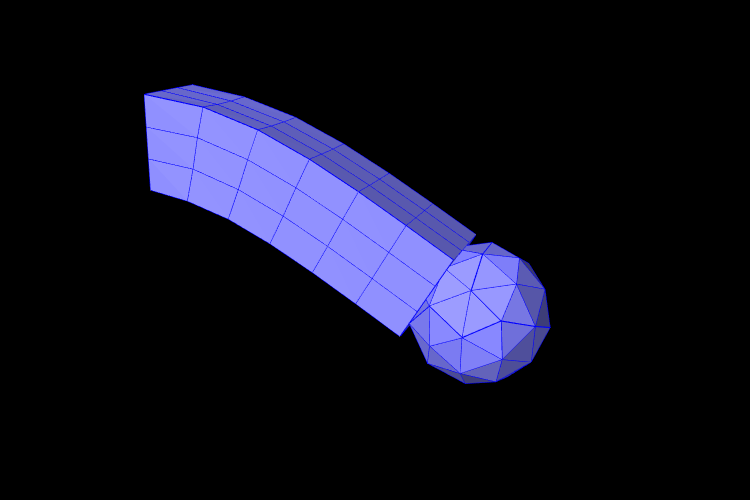
\includegraphics[width=\imglength]{images/FemBeamWithFemSphere}
	\caption{FemBeamWithFemSphere model loaded into ArtiSynth.}
	\label{fig:fem:beamwithfemsphere}
\end{figure}

The following model demonstrates how to attach two FEM models together:
\lstset{numbers=left}
\lstinputlisting{../../src/artisynth/demos/tutorial/FemBeamWithFemSphere.java}
\lstset{numbers=none}
This example can be found in 
{\tt artisynth.demos.tutorial.FemBeamWithFemSphere}.  The model extends 
{\tt FemBeam}, adding a finite element sphere and coupling them together.
The sphere is created and added on lines 18--28.  It is read from
TetGen-generated files using the 
\javaclass[artisynth.core.femmodels]{TetGenReader} class.  The model is then
scaled to match the dimensions of the current model, and transformed to the
right side of the beam.  To create attachments, the code first checks for 
any nodes that belong to the sphere that fall inside the beam using the
\javamethod[artisynth.core.femmodels]{FemModel3d.findContainingElement(Point3d)}
method (line 36), which returns the containing element if the point is inside
the model, or {\tt null} if the point is outside.  Internally, this spatial 
search uses a bounding volume hierarchy for efficiency (see 
\javaclass[maspack.geometry]{BVTree} and 
\javaclass[maspack.geometry]{BVFeatureQuery}).  If the point is contained
within the beam, then {\tt mech.attachPoint()}
is used to attach it to the nodes of the element (line 39).

\subsection{Nodal-based attachments}
\label{sec:fem:nodalAttachments}

The example of Section \ref{connectingTwoFems:sec} uses element-based
attachments to connect the nodes of one FEM to elements of another.
As mentioned above, element-based attachments assume that the attached
point is associated with a specific FEM model element. 
While this often gives good results, there are situations where it may
be desirable to distribute the connection more broadly among a larger
set of nodes. 

In particular, this is sometimes the case when connecting FEM models
to point-to-point springs. The end-point of such a spring may end up
exerting a large force on the FEM, and then if the number of nodes to
which the end-point is attached are too small, the resulting forces on
these nodes (Equation \ref{pointFemForces:eqn}) may end up being too
large. In other words, it may be desirable to distribute the spring's
force more evenly throughout the FEM model. 

To handle such situations, it is possible to create a {\it
nodal-based} attachment in which the nodes and weights are explicitly
specified. This involves explicitly creating a {\tt
PointFem3dAttachment} for the point or particle to be attached and the
specifying the nodes and weights directly,
%
\begin{lstlisting}[]
   PointFem3dAttachment ax = new PointFem3dAttachment (part);
   ax.setFromNodes (nodes, weights);
   mech.addAttachment (ax);
\end{lstlisting}
%
where {\tt nodes} and {\tt weights} are arrays of {\tt FemNode} and
{\tt double}, respectively. It is up to the application to determine
these.

\javaclass[artisynth.core.femmodels]{PointFem3dAttachment} provides
several methods for explicitly specifying nodes and weights. The
signatures for these include:
\begin{lstlisting}[]
  void setFromNodes (FemNode[] nodes, double[] weights)
  void setFromNodes (Collection<FemNode> nodes, VectorNd weights)
  boolean setFromNodes (Point3d pos, FemNode[] nodes)
  boolean setFromNodes (Point3d pos, Collection<FemNode> nodes)
\end{lstlisting}
The last two methods determine the weights automatically, using an
inverse-distance-based calculation in which each weight $w_k$
is initially computed as
%
\begin{equation}
w_k = \frac{d_{\text{max}}}{d_k + d_{max}}
\label{invDistWeights:eqn}
\end{equation}
%
where $d_k$ is the distance from node $k$ to {\tt pos} and
$d_{\text{max}}$ is the maximum distance. The weights are then
adjusted to ensure that they sum to one and that the weighted sum of
the nodes equals {\tt pos}. In some cases, the specified nodes
may not provide enough support for the last condition to be
met, in which case the methods return {\tt false}.

\subsection{Example: element vs. nodal-based attachments}

\begin{figure}[ht]
\centering
\setlengthLaTeXML{\imglength}{0.8\textwidth}{0.6\textwidth}
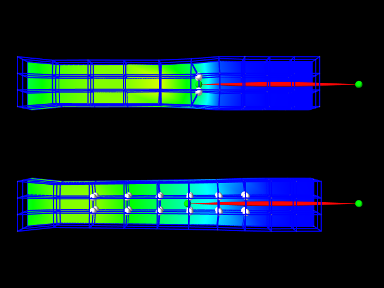
\includegraphics[width=\imglength]{images/PointFemAttachment}
\caption{PointFemAttachment loaded into ArtiSynth and run until stable.
The top and bottom models are connected to their springs using element
and nodal-based attachments, respectively.  The nodes associated with
each attachment are rendered as white spheres.}
\label{fig:fem:pointFemAttachment}
\end{figure}

The model demonstrating the difference between element and
nodal-based attachments is defined in
%
\begin{verbatim}
  artisynth.demos.tutorial.PointFemAttachment
\end{verbatim}
%
It creates two FEM models, each
with a single point-to-point spring attached to a particle at their
center. The model at the top ({\tt fem1} in the code below) is
connected to the particle using an element-based attachment, while the
lower model ({\tt fem2} in the code) is connected using a nodal-based
attachment with a larger number of nodes. Figure
\ref{fig:fem:pointFemAttachment} shows the result after the model is
run until stable. The element-based attachment results in
significantly higher deformation in the immediate vicinity around the
attachment, while for the nodal-based attachment, the deformation is
distributed much more evenly through the model.

The build method and some of the auxiliary code for this model is shown below.
Code for the other auxiliary methods, including {\tt addFem()},
{\tt addParticle()}, {\tt addSpring()}, and {\tt setAttachedNodesWhite()},
can be found in the actual source file.
\lstset{numbers=left}
\begin{lstlisting}[]
   // Filter to select only elements for which the nodes are entirely on the
   // positive side of the x-z plane.
   private class MyFilter extends ElementFilter {
      public boolean elementIsValid (FemElement e) {
         for (FemNode n : e.getNodes()) {
            if (n.getPosition().y < 0) {
               return false;
            }
         }
         return true;         
      }
   }

   // Collect and return all the nodes of a FEM model associated with a
   // set of elements specified by an array of element numbers
   private HashSet<FemNode3d> collectNodes (FemModel3d fem, int[] elemNums) {
      HashSet<FemNode3d> nodes = new HashSet<FemNode3d>();
      for (int i=0; i<elemNums.length; i++) {
         FemElement3d e = fem.getElements().getByNumber (elemNums[i]);
         for (FemNode3d n : e.getNodes()) {
            nodes.add (n);
         }
      }
      return nodes;
   }

   public void build (String[] args) {
      MechModel mech = new MechModel ("mech");
      addModel (mech);
      mech.setGravity (0, 0, 0); // turn off gravity

      // create and add two FEM beam models centered at the specified locations
      FemModel3d fem1 = addFem (mech,  0.0, 0.0,  0.25);
      FemModel3d fem2 = addFem (mech,  0.0, 0.0, -0.25);

      // reconstruct the FEM surface meshes so that they show only elements on
      // the positive side of the x-y plane. Also, set surface rendering to
      // show strain values.
      fem1.createSurfaceMesh (new MyFilter());
      fem1.setSurfaceRendering (SurfaceRender.Strain);
      fem2.createSurfaceMesh (new MyFilter());
      fem2.setSurfaceRendering (SurfaceRender.Strain);

      // create and add the particles for the point-to-point springs
      // that will apply forces to each FEM.
      Particle p1 = addParticle (mech,  0.9, 0.0,  0.25);
      Particle p2 = addParticle (mech,  0.9, 0.0, -0.25);
      Particle m1 = addParticle (mech,  0.0, 0.0,  0.25);
      Particle m2 = addParticle (mech,  0.0, 0.0, -0.25);

      // attach spring end-point to fem1 using an element-based marker
      mech.attachPoint (m1, fem1);

      // attach spring end-point to fem2 using a larger number of nodes, formed
      // from the node set for elements 22, 31, 40, 49, and 58. This is done by
      // explicitly creating the attachment and then setting it to use the
      // specified nodes
      HashSet<FemNode3d> nodes =
         collectNodes (fem2, new int[] { 22, 31, 40, 49, 58 });

      PointFem3dAttachment ax = new PointFem3dAttachment (m2);
      ax.setFromNodes (m2.getPosition(), nodes);
      mech.addAttachment (ax);

      // finally, create the springs
      addSpring (mech, /*stiffness=*/10000, p1, m1);
      addSpring (mech, /*stiffness=*/10000, p2, m2);

      // set the attachments nodes for m1 and m2 to render as white spheres
      setAttachedNodesWhite (m1);
      setAttachedNodesWhite (m2);
      // set render properties for m1
      RenderProps.setSphericalPoints (m1, 0.015, Color.GREEN);
   }
\end{lstlisting}
\lstset{numbers=none}
The {\tt build()} method begins by creating a {\tt MechModel} and then
adding to it two FEM beams (created using the auxiliary method {\tt
addFem()}. Rendering of each FEM model's surface is then set up to
show strain values ({\tt setSurfaceRendering()}, lines 41 and 43).
The surface meshes themselves are also redefined to exclude the
frontmost elements, allowing the strain values to be displayed closer
model centers. This redefinition is done using calls to {\tt
createSurfaceMesh()} (lines 40, 41) with a custom {\tt ElementFilter}
defined at lines 3-12.

Next, the end-point particles for the axial springs are created (using
the auxiliary method {\tt addParticle()}, lines
46-49), and particle {\tt m1} is attached to {\tt fem1} using {\tt
mech.attachPoint()} (line 52), which creates an element-based
attachment at the point's current location. Point {\tt m2} is then
attached to {\tt fem2} using a nodal-based attachment.  The nodes for
these are collected as the union of all nodes for a specufied set of
elements (lines 58-59, and the method {\tt collectNodes()} defined at
lines 16-25). These are then used to create a nodal-based attachment
(lines 61-63), where the weights are determined automatically using
the method associated with equation (\ref{invDistWeights:eqn}).

Finally, the springs are created (auxiliary method {\tt addSpring()},
lines 66-67), the nodes associated for each attachment are set to
render as white spheres ({\tt setAttachedNodesWhites()}, lines 70-71),
and the particles are set to render as green spheres.

To run this example in ArtiSynth, select {\sf All demos > tutorial >
PointFemAttachment} from the {\sf Models} menu. Running the model will
cause it to settle into the state shown in Figure
\ref{fig:fem:pointFemAttachment}. Selecting and dragging one of the
spring anchor points at the right will cause the spring tension to
vary and further illustrate the difference between the element
and nodal-based attachments.

\section{FEM markers}

Just as there are {\tt FrameMarker}s to act as anchor points on a frame or
rigid body (Section \ref{FrameMarkers:sec}), there are also {\tt FemMarker}s 
that can mark a point inside a finite element.  They are frequently used to 
provide anchor points for attaching springs and forces to a point inside 
an element, but can also be used for graphical purposes.

FEM markers are implemented by the class
\javaclass[artisynth.core.femmodels]{FemMarker}, which
is a subclass of
\javaclass[artisynth.core.mechmodels]{Point}.
They are essentially massless points that contain their own attachment
component, so when creating and adding a marker there is no need to
create a separate attachment component.

Within the component hierarchy, FEM markers are typically stored in
the {\tt markers} list of their associated FEM model. They can
be created and added using a code fragment of the form
%
\begin{lstlisting}[]
  FemMarker mkr = new FemMarker (1, 0, 0);
  mkr.setFromFem (fem); // attach to the nearest fem element
  fem.addMarker (mkr);  // add to fem
\end{lstlisting}
%
This creates a marker at the location $(1,0,0)$ (in world
coordinates), calls {\tt setFromFem()} to attach it to the nearest
element in the FEM model ( which is either the containing element or
the nearest element on the model's surface), and then adds it to the
{\tt markers} list.

If the marker's attachment has not already been set when {\tt
addMarker()} is called, then {\tt addMarker()} will call {\tt
setFromFem()} automatically. Therefore the above code fragment is
equivalent to the following:
%
\begin{lstlisting}[]
  FemMarker mkr = new FemMarker (1, 0, 0);
  fem.addMarker (mkr);
\end{lstlisting}
%
Alternatively, one may want to explicitly specify the nodes
associated with the attachment, as described in Section 
\ref{sec:fem:nodalAttachments}:
%
\begin{lstlisting}[]
  FemMarker mkr = new FemMarker (1, 0, 0);
  mkr.setFromNodes (nodes, weights);
  fem.addMarker (mkr);
\end{lstlisting}
%
There are a variety of methods available to set the attachment, mirroring
those available in the underlying base class {\tt PointFem3dAttachment}:
\begin{lstlisting}[]
  void setFromFem (FemModel3d fem)
  boolean setFromElement (FemElement3d elem)
  void setFromNodes (FemNode[] nodes, double[] weights)
  void setFromNodes (Collection<FemNode> nodes, VectorNd weights)
  boolean setFromNodes (FemNode[] nodes)
  boolean setFromNodes (Collection<FemNode> nodes)
\end{lstlisting}
The last two methods compute nodal weights automatically, as described
in Section \ref{sec:fem:nodalAttachments}, based on the marker's
currently assigned position. If the supplied nodes do not provide
sufficient support, then the methods return {\tt false}.

Another set of convenience methods are supplied by {\tt FemModel3d},
which combine these with the {\tt addMarker()} call:
%
\begin{lstlisting}[]
  void addMarker (FemMarker mkr, FemElement3d elem)
  void addMarker (FemMarker mkr, FemNode[] nodes, double[] weights)
  void addMarker (FemMarker mkr, Collection<FemNode> nodes, VectorNd weights)
  boolean addMarker (FemMarker mkr, FemNode[] nodes)
  boolean addMarker (FemMarker mkr, Collection<FemNode> nodes)
\end{lstlisting}
%
For example, one can do
%
\begin{lstlisting}[]
  FemMarker mkr = new FemMarker (1, 0, 0);
  fem.addMarker (mkr, nodes, weights);
\end{lstlisting}
%

Markers are often used to track movement within an FEM model.
For that, one can examine their positions and velocities,
as with any other particles, using the methods
%
\begin{lstlisting}[]
  Point3d getPosition();     // returns the current position
  Vectord getVelocity();     // returns the current velocity
\end{lstlisting}
%
The return values from these methods should not be
modified. Alternatively, when a 3D force $\f$ is applied to the
marker, it is distributed to the attached nodes according to the nodel
weights, as described in Equation \eqref{pointFemForces:eqn}.

\subsection{Example: attaching a FEM beam to a muscle}

\begin{figure}[ht]
	\centering
	\setlengthLaTeXML{\imglength}{0.8\textwidth}{0.6\textwidth}
	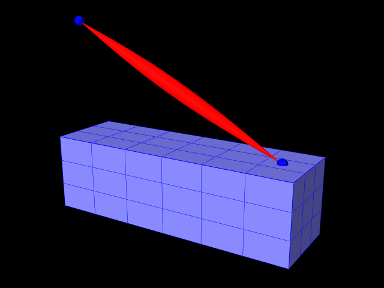
\includegraphics[width=\imglength]{images/FemBeamWithMuscle}
	\caption{FemBeamWithMuscle model loaded into ArtiSynth.}
	\label{fig:fem:beamwithmuscle}
\end{figure}

A complete application model that employs a fem marker as an anchor for a spring
is given below.
\lstset{numbers=left}
\lstinputlisting{../../src/artisynth/demos/tutorial/FemBeamWithMuscle.java}
\lstset{numbers=none}
This example can be found in {\tt artisynth.demos.tutorial.FemBeamWithMuscle}.
This model extends the {\tt FemBeam} example, adding a {\tt FemMarker} for the
spring to attach to.  The method {\tt createMarker(...)} on lines 29--35
is used to create and add a marker to the FEM.  Since the element is initially
set to {\tt null}, when it is added to the FEM, the model searches for the
containing or nearest element.  The loaded model is shown in Figure 
\ref{fig:fem:beamwithmuscle}.

% FemBeamWithMuscle

\section{Frame attachments}
\label{sec:fem:frameattachments}

It is also possible to attach frame components, including rigid
bodies, directly to FEM models, using the attachment component
\javaclass[artisynth.core.femmodels]{FrameFem3dAttachment}.
Analagously to
\javaclass[artisynth.core.femmodels]{PointFem3dAttachment}, the
attachment is implemented by connecting the frame to a set of FEM
nodes, and attachments can be either element-based or nodal-based.  The
frame's origin is computed in the same way as for point attachments,
using a weighted sum of node positions (Equation
\ref{pointFemAttachment:eqn}), while the orientation is computed using
a polar decomposition on a deformation gradient determined from either
element shape functions (for element-based attachments) or a
Procrustes type analysis using nodal rest positions (for nodal-based attachments).

An element-based attachment can be created using either a code fragment
of the form
%
\begin{lstlisting}[]
   FrameFem3dAttachment ax = new FrameFem3dAttachment(frame);
   ax.setFromElement (frame.getPose(), elem);
   mech.addAttachment (ax);
\end{lstlisting}
%
or, equivalently, the {\tt attachFrame()} method in {\tt MechModel}:
%
\begin{lstlisting}[]
   mech.attachFrame (frame, elem);
\end{lstlisting}
%
This attaches the frame {\tt frame} to the nodes of the FEM element
{\tt elem}. As with {\tt PointFem3dAttachment}, if the frame's origin
is not inside the element, it may not be possible to accurately
compute the internal nodal weights, in which case {\tt
setFromElement()} will return {\tt false}.

In order to have the appropriate element located automatically,
one can instead use
%
\begin{lstlisting}[]
   FrameFem3dAttachment ax = new FrameFem3dAttachment(frame);
   ax.setFromFem (frame.getPose(), fem);
   mech.addAttachment (ax);
\end{lstlisting}
%
or, equivalently, 
%
\begin{lstlisting}[]
   mech.attachFrame (frame, fem);
\end{lstlisting}
%

As with point-to-FEM attachments, it may be desirable to create a
nodel-based attachment in which the nodes and weights are not tied to
a specific element. The reasons for this are generally the same as
with nodal-based point attachments (Section
\ref{sec:fem:nodalAttachments}): the need to distribute the forces and
moments acting on the frame across a broader set of element nodes.
Also, element-based frame attachments use element shape functions to
determine the frame's orientation, which may produce slightly
asymmetric results if the frame's origin is located particularly close
to a specific node.

\javaclass[artisynth.core.femmodels]{FrameFem3dAttachment} provides
several methods for explicitly specifying nodes and weights. The
signatures for these include:
\begin{lstlisting}[]
  void setFromNodes (RigidTransform3d TFW, FemNode[] nodes, double[] weights)
  void setFromNodes (RigidTransform3d TFW, Collection<FemNode> nodes, 
                        VectorNd weights)
  boolean setFromNodes (RigidTransform3d TFW, FemNode[] nodes)
  boolean setFromNodes (RigidTransform3d TFW, Collection<FemNode> nodes)
\end{lstlisting}
Unlike their counterparts in {\tt PointFem3dAttachment}, the first two
methods also require the current desired pose of the frame {\tt TFW}
(in world coordinates).  This is because while nodes and weights will
unambiguously specify the frame's origin, they do not specify the
desired orientation.

\subsection{Example: attaching frames to a FEM beam}

\begin{figure}[ht]
	\centering
	\setlengthLaTeXML{\imglength}{0.8\textwidth}{0.6\textwidth}
	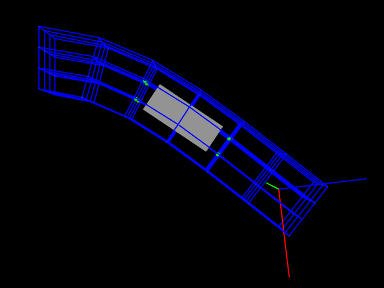
\includegraphics[width=\imglength]{images/FrameFemAttachment}
	\caption{FrameFemAttachment loaded into ArtiSynth and run until stable.}
	\label{fig:fem:frameFemAttachment}
\end{figure}

A model illustrating how to connect frames to a FEM model 
is defined in
%
\begin{verbatim}
  artisynth.demos.tutorial.FrameFemAttachment
\end{verbatim}
%
It creates a FEM beam, along with a rigid body block and a 
massless coordinate frame, that are then attached to the beam
using nodal and element-based attachments. The build method is shown below:
\lstset{numbers=left}
\begin{lstlisting}[]
   public void build (String[] args) {

      MechModel mech = new MechModel ("mech");
      addModel (mech);

      // create and add FEM beam 
      FemModel3d fem = FemFactory.createHexGrid (null, 1.0, 0.2, 0.2, 6, 3, 3);
      fem.setMaterial (new LinearMaterial (500000, 0.33));
      RenderProps.setLineColor (fem, Color.BLUE);
      RenderProps.setLineWidth (mech, 2);
      mech.addModel (fem);
      // fix leftmost nodes of the FEM
      for (FemNode3d n : fem.getNodes()) {
         if ((n.getPosition().x-(-0.5)) < 1e-8) {
            n.setDynamic (false);
         }
      }

      // create and add rigid body box
      RigidBody box = RigidBody.createBox (
         "box", 0.25, 0.1, 0.1, /*density=*/1000);
      mech.add (box);

      // create a basic frame and set its pose and axis length
      Frame frame = new Frame();
      frame.setPose (new RigidTransform3d (0.4, 0, 0, 0, Math.PI/4, 0));
      frame.setAxisLength (0.3);
      mech.addFrame (frame);

      mech.attachFrame (frame, fem); // attach using element-based attachment

      // attach the box to the FEM, using all the nodes of elements 31 and 32
      HashSet<FemNode3d> nodes = collectNodes (fem, new int[] { 22, 31 });
      FrameFem3dAttachment attachment = new FrameFem3dAttachment(box);
      attachment.setFromNodes (box.getPose(), nodes);
      mech.addAttachment (attachment);

      // render the attachment nodes for the box as spheres
      for (FemNode n : attachment.getNodes()) {
         RenderProps.setSphericalPoints (n, 0.007, Color.GREEN);
      }
   }
\end{lstlisting}
\lstset{numbers=none} 
Lines 3-22 create a {\tt MechModel} and populate it with an FEM beam
and a rigid body box. Next, a basic {\tt Frame} is created, with a
specified pose and an axis length of 0.3 (to allow it to be seen), and
added to the {\tt MechModel} (lines 25-28). It is then attached to the
FEM beam using an element-based attachment (line 30).  Meanwhile, the
box is attached to using a nodal-based attachment, created from all
the nodes associated with elements 22 and 31 (lines 33-36). Finally,
all attachment nodes are set to be rendered as green spheres (lines
39-41).

To run this example in ArtiSynth, select {\sf All demos > tutorial >
FrameFemAttachment} from the {\sf Models} menu. Running the model will
cause it to settle into the state shown in Figure
\ref{fig:fem:frameFemAttachment}. Forces can interactively
be applied to the attached block and frame using
pull manipulator, causing the FEM model to deform 
(see the section ``Pull Manipulator'' in the
\href{../uiguide/uiguide.html}{
ArtiSynth User Interface Guide}).

\subsection{Adding joints to FEM models}

The ability to connect frames to FEM models, as described in Section
\ref{sec:fem:frameattachments}, makes it possible to interconnect
different FEM models directly using joints, as described in Section
\ref{JointsAndConnectors:sec}. This is done internally by using {\tt
FrameFem3dAttachments} to connect frames C and D of the joint (Figure
\ref{jointExample:fig}) to their respective FEM models.

As indicated in Section \ref{CreatingJoints:sec}, most
joints have a constructor of the form
%
\begin{lstlisting}[]
  JointType (bodyA, bodyB, TDW);
\end{lstlisting}
%
that creates a joint connecting {\tt bodyA} to {\tt bodyB}, with the
initial pose of the D frame given (in world coordinates) by {\tt TDW}.
The same body and transform settings can be made on an existing joint
using the method \javamethodAlt{%
artisynth.core.mechmodels.BodyConnector.setBodies(ConnectableBody,,)}
{setBodies(bodyA, bodyB, TDW)}.  For these constructors and methods,
it is possible to specify FEM models for {\tt bodyA} and/or {\tt
bodyB}. Internally, the joint then creates a {\tt
FrameFem3dAttachment} to connect frame C and/or D of the joint (See
Figure \ref{jointExample:fig}) to the corresponding FEM model.

However, unlike joints involving rigid bodies or frames, there are no
associated $\T_{CA}$ or $\T_{DB}$ transforms (since there is no fixed
frame within an FEM to define such transforms).  Methods or
constructors which utilize $\T_{CA}$ or $\T_{DB}$ can therefore
not be used with FEM models.

\subsection{Example: two FEM beams connected by a joint}

\begin{figure}[ht]
	\centering
	\setlengthLaTeXML{\imglength}{0.8\textwidth}{0.6\textwidth}
	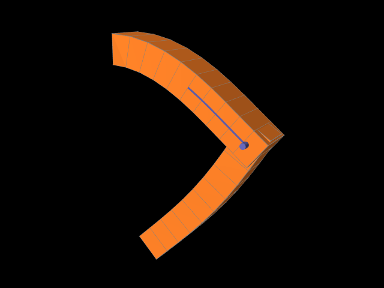
\includegraphics[width=\imglength]{images/JointedFemBeams}
	\caption{JointedFemBeams loaded into ArtiSynth and run until stable.}
	\label{fig:fem:jointFemBeams}
\end{figure}

A model connecting two FEM beams by a joint
is defined in
%
\begin{verbatim}
  artisynth.demos.tutorial.JointedFemBeams
\end{verbatim}
%
It creates two FEM beams and connects them via a special slotted-revolute
joint. The build method is shown below:
\lstset{numbers=left}
\begin{lstlisting}[]
   public void build (String[] args) {
      
      MechModel mech = new MechModel ("mechMod");
      addModel (mech);
      
      double stiffness = 5000;
      // create first fem beam and fix the leftmost nodes      
      FemModel3d fem1 = addFem (mech, 2.4, 0.6, 0.4, stiffness);
      for (FemNode3d n : fem1.getNodes()) {
         if (n.getPosition().x <= -1.2) {
            n.setDynamic(false);
         }
      }
      // create the second fem beam and shift it 1.5 to the right
      FemModel3d fem2 = addFem (mech, 2.4, 0.4, 0.4, 0.1*stiffness);
      fem2.transformGeometry (new RigidTransform3d (1.5, 0, 0));

      // create a slotted revolute joint that connects the two fem beams
      RigidTransform3d TDW = new RigidTransform3d(0.5, 0, 0, 0, 0, Math.PI/2);
      SlottedRevoluteJoint joint = new SlottedRevoluteJoint (fem2, fem1, TDW);
      mech.addBodyConnector (joint);
      
      // set ranges and rendering properties for the joint
      joint.setAxisLength (0.8);
      joint.setMinX (-0.5);
      joint.setMaxX (0.5);
      joint.setSlotWidth (0.61);
      RenderProps.setLineColor (joint, myJointColor);
      RenderProps.setLineWidth (joint, 3);
      RenderProps.setLineRadius (joint, 0.04);
   }
\end{lstlisting}
\lstset{numbers=none} Lines 3-16 create a {\tt MechModel} and
populates it with two FEM beams, {\tt fem1} and {\tt fem2}, using an
auxiliary method {\tt addFem()} defined in the model source file.  The
leftmost nodes of {\tt fem1} are set fixed. A {\tt
SlottedRevoluteJoint} is then created to interconnect {\tt fem1} and
{\tt fem2} at a location specified by {\tt TDW} (lines 19-21).  Lines
24-30 set some parameters for the joint, along with various render
properties.

To run this example in ArtiSynth, select {\sf All demos > tutorial >
JointedFemBeams} from the {\sf Models} menu. Running the model will
cause it drop and flex under gravity, as shown in 
\ref{fig:fem:jointFemBeams}. Forces can interactively
be applied to the beams using
pull manipulator 
(see the section ``Pull Manipulator'' in the
\href{../uiguide/uiguide.html}{
ArtiSynth User Interface Guide}).

\section{Incompressiblity}

FEM incompressibility within ArtiSynth is enforced by trying to ensure
that the volume of a FEM remains locally constant. This, in turn, is
accomplished by constraining nodal velocities so that the local volume change,
or \emph{divergence}, is zero (or close to zero). There are generally two
ways to do this:

\begin{itemize}
\item {\it Hard incompressibility}, which sets up explicit constraints on the
nodal velocities;
\item {\it Soft incompressibility}, which uses a restoring pressure based on a
potential field to try to keep the volume constant.
\end{itemize}

Both of these methods operate independently, and both can be used
either separately or together. Generally speaking, hard incompressibility
will result in incompressibility being more rigorously enforced, but
at the cost of increased computation time and (sometimes) less
stability. Soft incompressibility allows the application to control
the restoring force used to enforce incompressibility, usually by
adjusting the value of the \emph{bulk modulus} material property.  As
the bulk modulus is increased, soft incompressibility starts to act
more like `hard' incompressibility, with an infinite bulk modulus
corresponding to perfect incompressibilty. However, very large bulk
modulus values will generally produce stability problems.

\subsection{Volume regions and locking}
\label{VolumeRegions:sec}

Both hard and soft incompressibility can be applied to different
regions of local volume. From larger to smaller, these regions are:

\begin{itemize}
\item {\it Nodal} - the local volume surrounding each node;
\item {\it Element} - the volume of each element;
\item {\it Full} - the volume at each integration point.
\end{itemize}

Element-based incompressibility is the standard method generally seen
in the literature. However, it tends not to work well for
tetrahedral meshes, because constraining the volume of each tet in a
tetrahedral mesh tends to over constrain the system. This is because
the number of tets in a large tetrahedral mesh is often $O(5 n)$,
where $n$ is the number of nodes, and so putting a volume constraint
on each element may result in $O(5 n)$ constraints, which exceeds the
$3 n$ degrees of freedom (DOF) in the FEM. This overconstraining results in an
artificially increased stiffness known as \emph{locking}. Because of
locking, for tetrahedrally based meshes it may be better to use
nodal-based incomressibility, which creates a single volume constraint
around each node, resulting in only $n$ constraints, leaving $2 n$ DOF
to handle the remaining deformation.  However, nodal-based
imcompressibility is computationally more costly than element-based
and may not be as stable.

Generally, the best solution for incompressible problems is to use
element-based incompressibility with a mesh consisting of hexahedra,
or primarily hexahedra and a mix of other elements (the latter
commonly being known as a \emph{hex dominant} mesh). For hex-based
meshes, the number of elements is roughly equal to the number of
nodes, and so adding a volume constraint for each element imposes $n$
constraints on the model, which (like nodal incompressibility)
leaves $2 n$ DOF to handle the remaining deformation.

Full incompressibility tries to control the volume at each
integration point within each element, which almost always results in
a large number of volumetric constraints and hence locking. It is
therefore not commonly used and is provided mostly for debugging and
diagnostic purposes.

\subsection{Hard incompressibility}
\label{HardIncomp:sec}

Hard incompressibility is controlled by the {\sf incompressible}
property of the FEM, which can be set to one of the following values
of the enumerated type {\tt FemModel.IncompMethod}:

\begin{description}

\item[OFF] No hard incompressibility enforced.

\item[ELEMENT] Element-based hard incompressibility enforced
(Section \ref{VolumeRegions:sec}).

\item[NODAL] Nodal-based hard incompressibility enforced
(Section \ref{VolumeRegions:sec}).

\item[AUTO] Selects either {\tt ELEMENT} or {\tt NODAL},
with the former selected if the number of elements is less than or
equal to the number of nodes.

\item[ON] Same as {\tt AUTO}.

\end{description}

Hard incompressibility uses explicit constraints on the nodal
velocities to enforce the incompressibilty, which increases
computational cost. Also, if the number of constraints is too large,
{\it perturbed pivot} errors may be encountered by the solver.
However, hard incompressibility can in principle handle situtations
where complete incompressibility is required. It is equivalent to the
mixed u-P formulation used in commercial FEM codes (such as ANSYS),
and the Lagrange multipliers computed for the constraints are pressure
impulses.

Hard incompressibility can be applied in addition to soft
incompressibility, in which case it will provide additional
incompressibility enforcement on top of that provided by the latter.
It can also be applied to linear materials, which are not themselves
able to emulate true incompressible behavior
(Section \ref{IncompLinearMaterials:sec}).

\subsection{Soft incompressibility}
\label{SoftIncomp:sec}

Soft incompressibility enforces incompressibility using a restoring
pressure that is controlled by a volume-based energy potential. It is
only available for FEM materials that are subclasses of
\javaclass[artisynth.core.materials]{IncompressibleMaterial}.
The energy potential $U(J)$ is a function of the determinant $J$ of the
deformation gradient, and is scaled by the material's {\it bulk modulus}
$\kappa$. The restoring pressure $p$ is given by
%
\begin{equation}
p = \frac{\partial U}{\partial J}.
\end{equation}
%
Different potentials can be selected by setting the {\sf bulkPotential}
property of the incompressible material, whose value is an instance of
{\tt IncompressibleMaterial.BulkPotential}.  Currently
there are two different potentials:

\begin{description}

\item[QUADRATIC] The potential and associated pressure
are given by
%
\begin{equation}
U(J) = \frac{1}{2}\kappa (J - 1)^2, \quad p = \kappa (J - 1).
\end{equation}
%

\item[LOGARITHMIC]
The potential and associated pressure
are given by
%
\begin{equation}
U(J) = \frac{1}{2}\kappa (\ln J)^2, \quad p = \kappa \frac{\ln J}{J}
\end{equation}
%

\end{description}

The default potential is {\tt QUADRATIC}, which may provide slightly
improved stability characteristics.  However, we have not noticed
significant differences between the two potentials in practice.

How soft incompressibility is applied within a FEM model is controlled
by the FEM's {\sf softIncompMethod} property, which can be set to one
of the following values of the enumerated type {\tt
FemModel.IncompMethod}:

\begin{description}

\item[ELEMENT] Element-based soft incompressibility enforced
(Section \ref{VolumeRegions:sec}).

\item[NODAL] Nodal-based soft incompressibility enforced
(Section \ref{VolumeRegions:sec}).

\item[AUTO] Selects either {\tt ELEMENT} or {\tt NODAL},
with the former selected if the number of elements is less than or
equal to the number of nodes.

\item[FULL] Incompressibility enforced at each integration point
(Section \ref{VolumeRegions:sec}).

\end{description}

\subsection{Incompressibility and linear materials}
\label{IncompLinearMaterials:sec}

Within a linear material, incompressibility is controlled by Poisson's
ratio $\nu$, which for isotropic materials can assume a value in the
range $[-1, 0.5]$. This specifies the amount of transvere contraction
(or expansion) exhibited by the material as it compressed or extended
along a particular direction. A value of $0$ allows the material to be
compressed or extended without any transverse contraction or
expansion, while a value of $0.5$ in theory indicates a perfectly
incompressible material. However, setting $\nu = 0.5$ in practice
causes a division by zero, so only values close to 0.5 (such as 0.49)
can be used. 

Moreover, the incompressibility only applies to small displacements,
so that even with $\nu = 0.49$ it is still possible to squash a linear
FEM completely flat if enough force is applied. If true incompressible
behavior is desired with a linear material, then one must also use
hard incompressibility (Section \ref{HardIncomp:sec}).

\subsection{Using incompressibility in practice}

As mentioned above, when modeling incompressible models, we have found
that the best practice is to use, if possible, either a hex or
hex-dominant mesh, along with element-based incompressibility.

Hard incompressibility allows the handling of full incompressibility
but at the expense of greater computational cost and often less
stability. When modeling biomechanical materials, it is often
permissible to use only soft incompressibility, partly since
biomechanical materials are rarely completely incompressible.  When
implementing soft incompressibility, it is common practice to set the
bulk modulus to something like 100 times the other (deviatoric)
stiffnesses of the material.

We have found stability behavior to be complex, and while hard
incompressibilty often results in less stable behavior, this is not
always the case: in some situations the stronger enforcement afforded
by hard incompressibility actually improves stabilty.

\section{Muscle activated FEM models}
\label{sec:fem:muscle}

Finite element muscle models are an extension to regular FEM models.  As such,
everything previously discussed for regular FEM models also applies to FEM
muscles.  Muscles have additional properties that allow them to contract when 
activated.  There are two types of muscles supported:
\begin{description}
\item[Fibre-based:] Point-to-point muscle fibres are embedded in the model.
\item[Material-based:] An auxiliary material is added to the constitutive law
    to embed muscle properties. 
\end{description}
In this section, both types will be described.

\subsection{FemMuscleModel}

The main class for FEM-based muscles is 
\javaclass[artisynth.core.femmodels]{FemMuscleModel}, a subclass 
of \javaclass[artisynth.core.femmodels]{FemModel3d}.  It differs from a basic
FEM model in that it has the new property
\begin{center}
	\begin{tabular}{|ll|}
		\hline
		Property & Description\\
		\hline
		{\tt muscleMaterial} & An object that adds an activation-dependent
		                       `muscle' term to the \emph{constitutive law}.\\
		\hline
	\end{tabular}
\end{center}
This is a delegate object of type 
\javaclass[artisynth.core.materials]{MuscleMaterial} that computes activation-%
dependent stress and stiffness in the muscle. In addition to this property, 
{\tt FemMuscleModel} adds two new lists of subcomponents:
\begin{description}
   \item[{\tt bundles}]\mbox{}\\
   Groupings of muscle sub-units (fibres or elements) that can be activated.

   \item[{\tt exciters}]\mbox{}\\
   Components that control the activation of a set of bundles or other exciters.
\end{description}

\paragraph{Bundles}
\ifLaTeXML{\newline}

Muscle bundles allow for a muscle to be partitioned into separate groupings
of fibres/elements, where each bundle can be activated independently.  They 
are implemented in the class \javaclass[artisynth.core.femmodels]{MuscleBundle}.
Bundles have three key properties:
\begin{center}
	\begin{tabular}{|ll|}
		\hline
		Property & Description\\
		\hline
		{\tt excitation} & Activation level of the muscle,  $a\in[0, 1]$.\\
		{\tt fibresActive} & Enable/disable ``fibre-based'' muscle components.\\
		{\tt muscleMaterial} & An object that adds an activation-dependent
		                       `muscle' term to the \emph{constitutive law}.\\
		\hline
	\end{tabular}
\end{center}
The {\tt excitation} property controls the level of muscle activation, with zero 
being no muscle action, and one being fully activated.  The {\tt fibresActive} 
property is a boolean variable that controls whether or not to treat any 
contained fibres as point-to-point-like muscles (``fibre-based'').  If false, 
the fibres are ignored.  The third property, {\tt muscleMaterial}, allows for a 
{\tt MuscleMaterial} to be specified per bundle.  By default, its value is 
inherited from {\tt FemMuscleModel}.

Once a muscle bundle is created, muscle sub-units must be assigned to it.  These
are either point-to-point fibres, or material-based muscle element descriptors.
The two types will be covered in Sections \ref{sec:fem:fibremuscle} and
\ref{sec:fem:materialmuscle}, respectively.

\paragraph{Exciters}
\ifLaTeXML{\newline}

Muscle exciters enable you to simultaneously activate a group of ``excitation 
components''.  This includes: point-to-point muscles, muscle bundles, muscle
fibres, material-based muscle elements, and other muscle exciters.  Components 
that can be excited all implement the 
\javaclass[artisynth.core.mechmodels]{ExcitationComponent}
interface.  To add or remove a component to the exciter, use
\begin{lstlisting}[]
  addTarget (ExcitationComponent ex);    // adds a component to the exciter
  addTarget (ExcitationComponent ex,     // adds a component with a gain factor
  	   double gain);   
  removeTarget (ExcitationComponent ex); // removes a component
\end{lstlisting}
If a gain factor is specified, the activation is scaled by the gain for that
component.

\subsection{Fibre-based muscles}
\label{sec:fem:fibremuscle}

In fibre-based muscles, a set of point-to-point muscle fibres are added between
FEM nodes or markers.  Each fibre is assigned an 
\javaclass[artisynth.core.materials]{AxialMuscleMaterial}, just like for 
regular point-to-point muscles (Section \ref{sec:mechii:musclematerials}).  Note
that these muscle materials typically have a ``rest length'' property, that will
likely need to be adjusted for each fibre.  Once the set of fibres are added
to a {\tt MuscleBundle}, they need to be enabled.  This is done by setting
the {\tt fibresActive} property of the bundle to {\tt true}.

Fibres are added to a {\tt MuscleBundle} using one of the functions:
\begin{lstlisting}[]
addFibre( Muscle muscle );              // adds a point-to-point fibre
Muscle addFibre( Point p0, Point p1,    // creates and adds a fibre
	 AxialMuscleMaterial mat);
\end{lstlisting}
The latter returns the newly created {\tt Muscle} fibre.  
The following code snippet demonstrates how to create a fibre-based 
{\tt MuscleBundle} and add it to a FEM muscle.
\lstset{numbers=left}
\begin{lstlisting}[]
// Create a muscle bundle
MuscleBundle bundle = new MuscleBundle("fibres");
Point3d[] fibrePoints = ...   //create a sequential list of points

// Add fibres
Point pPrev = fem.addMarker(fibrePoints[0]);    // create a FEM marker
for (int i=1; i<=fibrePoints.length; i++) {
   Point pNext = fem.addMarker(fibrePoint[i]);

   // Create fibre material
   double l0 = pNext.distance(pPrev);           // rest length
   AxialMuscleMaterial fibreMat = 
         new BlemkerAxialMuscle(
               1.4*l0, l0, 3000, 0, 0);

   // Add a fibre between pPrev and pNext
   bundle.addFibre(pPrev, pNext, fibreMat);     // add fibre to bundle
   pPrev = pNext;
}

// Enable use of fibres (default is disabled)
bundle.setFibresActive(true);
fem.addMuscleBundle(bundle);                    // add the bundle to fem
\end{lstlisting}
\lstset{numbers=none}

In these fibre-based muscles, force is only exerted between the anchor
points of the fibres; it is a discrete approximation.  These models
are typically more stable than material-based ones.

\subsection{Material-based muscles}
\label{sec:fem:materialmuscle}

In material-based muscles, the constitutive law is augmented with additional
terms to account for muscle-specific properties.  This is a continuous 
representation within the model.  

The basic building block for a material-based muscle bundle is a 
\javaclass[artisynth.core.femmodels]{MuscleElementDesc}.  This object contains
a reference to a {\tt FemElement3d}, a {\tt MuscleMaterial}, and either a
single direction or set of directions that specify the direction of 
contraction.  If a single direction is specified, then it is assumed the
entire element contracts in the same direction.  Otherwise, a direction
can be specified for each \emph{integration point} within the element.  A
{\tt null} direction signals that there is no muscle at the corresponding
point.  This allows for a sub-element resolution for muscle definitions. The 
positions of integration points for a given element can be obtained with:
\begin{lstlisting}[]
// loop through all integration points for a given element
for ( IntegrationPoint3d ipnt : elem.getIntegrationPoints() ) {
	Point3d curPos = new Point3d();
	Point3d restPos = new Point3d();
	ipnt.computePosition (curPos, elem);          // computes current position
	ipnt.computeRestPosition (restPos, elem);     // computes rest position
}
\end{lstlisting} 
By default, the {\tt MuscleMaterial} is inherited from the bundle's 
{\tt material} property.  Supported muscle materials include:
\javaclass[artisynth.core.materials]{GenericMuscle}, 
\javaclass[artisynth.core.materials]{BlemkerMuscle}, and 
\javaclass[artisynth.core.materials]{FullBlemkerMuscle}.  The Blemker-type
materials are based on \cite{blemker:2005:muscle}.  {\tt BlemkerMuscle} only
uses the muscle-specific terms (since a base material is provided the 
underlying FEM model), whereas {\tt FullBlemkerMuscle} adds all terms described in 
the aforementioned paper.

Elements can be added to a muscle bundle using one of the methods:
\begin{lstlisting}[]
// Adds a muscle element
addElement (MuscleElementDesc elem);          
// Creates and adds a muscle element
MuscleElementDesc addElement (FemElement3d elem, Vector3d dir);     
// Sets a direction per integration point
MuscleElementDesc addElement (FemElement3d elem, Vector3d[] dirs);  
\end{lstlisting}

The following snippet demonstrates how to create and add a material-based
muscle bundle:
\lstset{numbers=left}
\begin{lstlisting}[]
// Create muscle bundle
MuscleBundle bundle = new MuscleBundle("embedded");

// Muscle material
MuscleMaterial muscleMat = new BlemkerMuscle(
      1.4, 1.0, 3000, 0, 0);
bundle.setMuscleMaterial(muscleMat); 

// Muscle direction
Vector3d dir = Vector3d.X_UNIT;

// Add elements to bundle
for (FemElement3d elem : beam.getElements()) {
   bundle.addElement(elem, dir);
}

// Add bundle to model      
beam.addMuscleBundle(bundle);
\end{lstlisting}
\lstset{numbers=none}

\subsection{Example: comparison with two beam examples}

\begin{figure}[ht]
	\centering
	\setlengthLaTeXML{\imglength}{0.8\textwidth}{0.6\textwidth}
	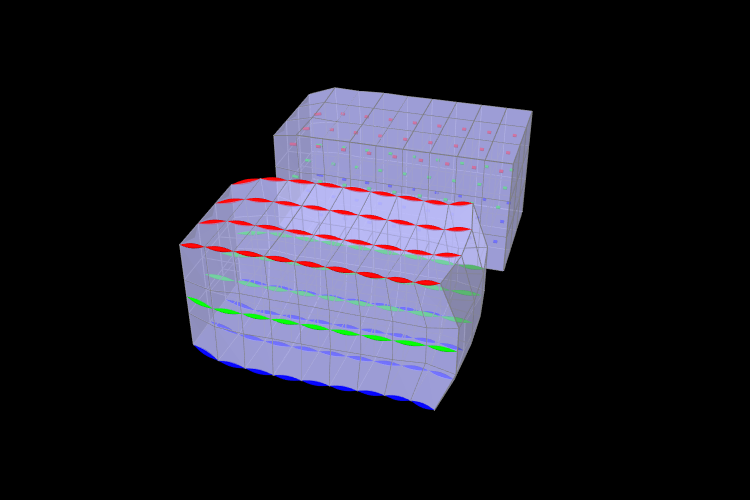
\includegraphics[width=\imglength]{images/FemMuscleBeamsContracted}
	\caption{FemMuscleBeams model loaded into ArtiSynth.}
	\label{fig:fem:musclebeams}
\end{figure}

% FemMuscleBeams
An example comparing a fibre-based and a material-based muscle is shown 
in Figure \ref{fig:fem:musclebeams}.  The code can be found in 
{\tt artisynth.demos.tutorial.FemMuscleBeam}.  There are two 
{\tt FemMuscleModel} beams in the model: one fibre-based, and one 
material-based.  Each has three muscle bundles: one at the top (red),
one in the middle (green), and one at the bottom (blue).  In the figure,
both muscles are fully activated.  Note the deformed shape of the beams.
In the fibre-based one, since forces only act between point on the fibres,
the muscle seems to bulge.  In the material-based muscle, the entire
continuous volume contracts, leading to a uniform deformation.  

Material-based muscles are more realistic.  However, this often comes at the cost
of stability.  The added terms to the constitutive law are highly non-linear,
which may cause numerical issues as elements become highly contracted or
highly deformed.  Fibre-based muscles are, in general, more stable.  However,
they can lead to bulging and other deformation artifacts due to their discrete
nature.

\section{Collisions}
\label{sec:fem:collision}

As described in Section \ref{sec:mechii:collisions}, collisions can be enabled 
for any class that implements the 
\javaclass[artisynth.core.mechmodels]{Collidable} interface.  Both 
\javaclass[artisynth.core.femmodels]{FemModel3d} and 
\javaclass[artisynth.core.femmodels]{FemMeshComp} implement 
\javaclass[artisynth.core.mechmodels]{Collidable}.  {\tt FemModel3d}
will use its surface mesh as the collision surface.  A {\tt FemMeshComp} will use
its underlying mesh structure.  At present, only meshes of type 
\javaclass[maspack.geometry]{PolygonalMesh} are supported.

Since {\tt FemMeshComp} is also a {\tt Collidable}, this means we can enable 
collisions with any embedded mesh inside a FEM.  Any forces resulting from
the collision are then automatically transfered back to the underlying nodes 
of the model using Equation \eqref{pointFemForces:eqn}.

\subsection{Example: FEM collisions}

\begin{figure}[ht]
	\centering
	\setlengthLaTeXML{\imglength}{0.8\textwidth}{0.6\textwidth}
	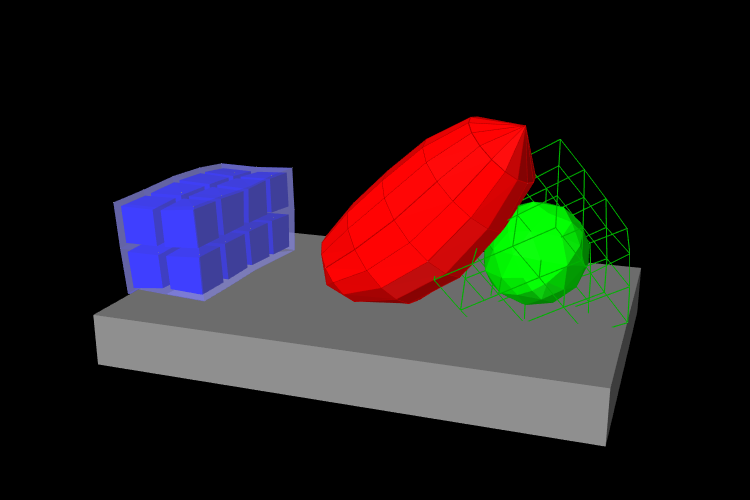
\includegraphics[width=\imglength]{images/FemCollisions}
	\caption{FemCollisions model loaded into ArtiSynth.}
	\label{fig:fem:collisions}
\end{figure}

An example of FEM collisions is shown in Figure \ref{fig:fem:collisions}.
The full source code can be found in the ArtiSynth repository under
{\tt artisynth.demos.tutorial.FemCollisions}.  The collision-enabling
code is as follows:
\begin{lstlisting}[]
// Set up collisions
mech.setCollisionBehavior(ellipsoid, beam, true);   // beam-ellipsoid
mech.setCollisionBehavior(ellipsoid, table, true);  // ellipsoid-table
mech.setCollisionBehavior(table, beam, true);       // beam-table

FemMeshComp embeddedSphere = block.getMeshComp("embedded");      // get embedded FemMeshComp
mech.setCollisionBehavior(embeddedSphere, table, true);      // sphere-table
mech.setCollisionBehavior(ellipsoid, embeddedSphere, true);  // sphere-ellipsoid   
\end{lstlisting}
Notice in the figure that the surface of the green block passes through
the table and ellipsoid; only the embedded sphere has collisions enabled.

\section{Rendering and Visualizations}
\label{sec:fem:rendering}

In addition to the standard {\tt RenderProps} that control how the
nodes and surfaces appear, finite element models and their sub-components
have a few additional properties that affect rendering.  Some of these
are listed in Table \ref{tbl:fem:rendering}.

\begin{table}[ht]
	\centering
	\caption{FEM-specific rendering properties} \label{tbl:fem:rendering}
	\begin{tabular}{lp{0.5\textwidth}}
		\hline\hline
		Property & Description\\
		\hline
	   {\tt elementWidgetSize} & size of element to render $\in [0,1]$\\
	   {\tt directionRenderLen} & relative length to draw fibre direction indicator $\in [0, 1]$\\
	   {\tt directionRenderType} & where to draw directions: {\tt ELEMENT}, {\tt INTEGRATION\_POINT}\\
	   {\tt surfaceRendering} & how to render surface: {\tt None}, {\tt Shaded}, {\tt Stress}, {\tt Strain}\\
	   {\tt stressPlotRange} & range of values for stress/strain plot\\
	   {\tt stressPlotRanging} & how to determine stress/strain plot range: {\tt Auto}, {\tt Fixed}\\
	   {\tt colorMap} & delegate object controlling the map of stress/strain values to color\\
	   \hline
	\end{tabular}
\end{table}

The property {\tt elementWidgetSize} applies only to 
\javaclass[artisynth.core.femmodels]{FemModel3d} and
\javaclass[artisynth.core.femmodels]{FemElement3d}.  It specifies the scale to
draw each element volume.  For instance, the blue beam in Figure \ref{fig:fem:collisions}
uses a widget size of 0.8, resulting in a mosaic-like pattern.

The next two properties in Table \ref{tbl:fem:rendering} apply to the muscle classes 
\javaclass[artisynth.core.femmodels]{FemMuscleModel}, 
\javaclass[artisynth.core.femmodels]{MuscleBundle}, and
\javaclass[artisynth.core.femmodels]{MuscleElementDesc}.
When {\tt directionRenderLen > 0}, lines are drawn inside elements to indicate fibre
directions.  If {\tt directionRenderType = ELEMENT}, then one line is drawn per
element indicating the average contraction direction.  If 
{\tt directionRenderType = INTEGRATION\_POINT}, a separate direction line is drawn 
per point.

The last four properties apply to 
\javaclass[artisynth.core.femmodels]{FemModel3d} and 
\javaclass[artisynth.core.femmodels]{FemMeshComp}.
They control how the surface is colored.  This can be used to enable stress/strain
visualizations.  The property {\tt surfaceRendering} sets what to draw:\\
\medskip
\begin{tabular}{lll}
& {\tt None} & no surface\\
& {\tt Shaded} & the face color specified by the mesh's {\tt RenderProps}\\
& {\tt Stress} & the von Mises stress\\
& {\tt Strain} & the von Mises strain
\end{tabular}
\medskip\\
The {\tt stressPlotRange} controls the range of values to use when plotting 
stress/strain.  Values outside this range are truncated.  The {\tt colorMap}
is a delegate object that converts those stress and strain values to colors.
Various types of maps exist, including 
\javaclass[maspack.render.color]{GreyscaleColorMap},
\javaclass[maspack.render.color]{HueColorMap},
\javaclass[maspack.render.color]{RainbowColorMap}, and
\javaclass[maspack.render.color]{JetColorMap}.  These all implement the
\javaclass[maspack.render.color]{ColorMap} interface.

To display values corresponding to colors, a 
\javaclass[artisynth.core.renderables]{ColorBar} needs to be added to the 
{\tt RootModel}.  Color bars are general {\tt Renderable} objects that are
only used for visualizations.  They are added to the display using the
\begin{lstlisting}[]
addRenderable (Renderable r);
\end{lstlisting}
method in {\tt RootModel}.  Color bars also have a {\tt ColorMap} associated
with it.  The following functions are useful for controlling its visualization:
\begin{lstlisting}[]
setNumberFormat ( String fmtStr );    // C-like numeric format specification
populateLabels ( double min, double max, int tick );     // initialize labels
updateLabels ( double min, double max );                 // update existing labels

setColorMap ( ColorMap map );                            // set color map

// Control position/size of the bar
setNormalizedLocation (double x, double y, double width, double height);
setLocationOverride (double x, double y, double width, double height)
\end{lstlisting}
The normalized location specifies sizes relative to the screen size 
(1 = screen width/height).  The location override, if values are non-zero,
will override the normalized location, specifying values in absolute pixels.
Negative values for position correspond to distances from the left/top.
For instance,
\begin{lstlisting}[]
setNormalizedLocation(0, 0.1, 0, 0.8);  // set relative positions
setLocationOverride(-40, 0, 20, 0);     // override with pixel lengths
\end{lstlisting}
will create a bar that is 10\% up from the bottom of the screen, 40 pixels from
the right edge, with a height occupying 80\% of the screen, and width 20 pixels.

Note that the color bar is not associated with any mesh or finite element model.
Any synchronization of colors and labels must be done manually by the developer.
It is recommended to do this in the {\tt RootModel}'s {\tt prerender(...)} method,
so that colors are updated every time the model's rendering configuration changes.

\subsection{Example: stress and strain plotting}

\begin{figure}[ht]
	\centering
	\setlengthLaTeXML{\imglength}{0.8\textwidth}{0.6\textwidth}
	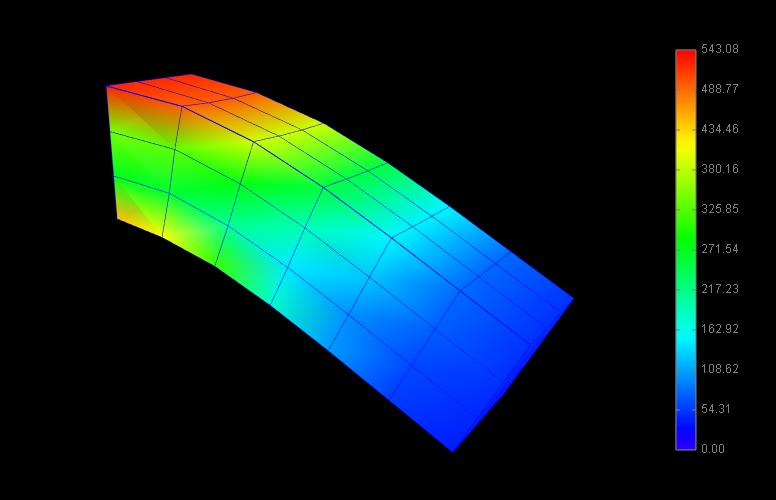
\includegraphics[width=\imglength]{images/FemBeamColored}
	\caption{FemBeamColored model loaded into ArtiSynth.}
	\label{fig:fem:beamcolored}
\end{figure}

The following model extends {\tt FemBeam} to render stress, with an added 
color bar.  The loaded model is shown in Figure \ref{fig:fem:beamcolored}.
\lstset{numbers=left}
\lstinputlisting{../../src/artisynth/demos/tutorial/FemBeamColored.java}
\lstset{numbers=none}
